\documentclass{article}
\usepackage{amsmath}
\usepackage{graphicx} % Required for inserting images
\usepackage{listings}
\usepackage{xcolor}
\usepackage[top=1in, bottom=1in, left=1.2in, right=1.2in]{geometry}
\usepackage{indentfirst}
\usepackage{url}
\usepackage{hyperref}
\usepackage{booktabs}



\title{Maximizing Dealership Profitability through Combinatorial Optimization of Parking Lot Allocation}
\author{Leo Lin, Jiaming Chang, Kevin Jia, Tim Lee}
\date{March 2025}

\begin{document}
    
\maketitle

\section{Abstract}

Every car dealership needs to optimize the inventory allocation that maximizes revenue and profit when operating within the constraints of limited parking space. This project aims to model the problem through the application of combinatorial optimization to the knapsack problem, given a limited parking lot capacity, each vehicle’s size, expected sale, and relative carbon tax must be considered when selecting the optimal subset of vehicles. The goal of the project is to maximize the overall sale value, which ensures the total park area does not exceed the available space. We develop an optimization framework to enhance the decision-making of vehicle resale, to contribute to the broader field of combinatorial programming research, providing future insights and predictions into efficient resource allocation under spatial and financial limitations.


\section{Introduction}

Optimizing inventory allocation is a fundamental challenge in the automotive industry, particularly for dealerships that must manage limited parking space while maximizing revenue and profit. Unlike traditional retail businesses, which store products in large warehouses without spatial constraints, dealerships must operate within a fixed physical space. This limitation requires dealership staff to strategically select which vehicles to display and resell. Since each vehicle differs in size, expected sale value, and potential environmental costs (e.g., carbon tax), determining the most profitable allocation within a dealership’s limited parking lot presents a combinatorial optimization problem.

This scenario can be effectively modeled using the Knapsack Problem (KP), a classical combinatorial optimization problem in operations research. The Knapsack Problem involves selecting a subset of items, each with an associated weight and value, such that the total weight remains within a given capacity while maximizing the overall value. In the context of a dealership, the weight corresponds to each vehicle’s spatial occupation in the parking lot, while the value represents its sale price. Additionally, environmental regulations impose carbon tax costs, introducing an additional economic factor that influences the optimization process. The objective is to determine the most profitable combination of vehicles that can fit within the available parking space while considering economic and regulatory constraints.

To make the problem tractable, we introduce the following assumptions:
\begin{itemize}
    \item Due to surtaxes on importing plug-in vehicles, we assume that the there will be no cars in the selection that are both electric (hybrid, plug-in hybrid) and imported.
    \item The dealership sources vehicles from car auctions and car rental companies, where wholesale data is generally unavailable and highly variable. Therefore, we assume that only auctioned cars with prices below resale value would be considered, and buying prices are generated based on car type. However, a dealership with access to auction data can adjust the buying prices as needed when running this optimization model.
    \item We assume that selected vehicles will be sold at market value, meaning that "market value" and "resale value" are interchangeable terms.
\end{itemize}


For this project, we employ the \href{https://www.kaggle.com/datasets/taeefnajib/used-car-price-prediction-dataset/data}{Used Car Price Prediction Dataset} from Kaggle, with modifications to enhance clarity and facilitate algorithmic interpretation. Out of the original 12 features, we removed 8 that were irrelevant to our problem and added 4 new features to better simulate the data available to a dealership’s decision-making process. A detailed discussion of data pre-processing and analysis is presented in later sections.





\section{Problem Statement}
Car dealerships must carefully manage their inventory to \textbf{maximize profitability} while operating within constraints related to space, budget, and environmental regulations. The dealership's parking lot has a \textbf{fixed capacity}, limiting the number of vehicles that can be displayed at any given time. As a result, selecting the optimal set of vehicles for display is crucial to achieving the highest possible resale profit.  

Beyond space limitations, dealerships must also account for \textbf{vehicle acquisition costs and environmental taxation}. High-emission vehicles incur additional \textbf{carbon tax costs}, which directly impact overall profitability. The challenge, therefore, is to develop an \textbf{optimization model} that determines the \textbf{most profitable subset of vehicles} to display while ensuring compliance with parking space constraints and taxation policies.  

This problem can be formulated as a \textit{combinatorial optimization task}, where each vehicle has specific attributes, including \textbf{purchase cost, resale value, size, and associated carbon tax}. The objective is to select a subset of vehicles that \textbf{maximizes total resale value} while ensuring that:  
\begin{enumerate}
    \item The \textbf{total occupied space} does not exceed the dealership’s parking lot capacity.
    \item The \textbf{total purchase cost} does not exceed the allocated budget.
    \item Additional costs, such as \textbf{licensing fees for imported vehicles} and \textbf{infrastructure upgrades for hybrid vehicles}, are accounted for.
\end{enumerate}

To address this problem, we propose 2 \textbf{mathematical optimization frameworks} that enables dealerships to make \textbf{data-driven inventory selection decisions}. By solving this optimization problem, dealerships can enhance revenue potential while effectively managing costs and regulatory constraints. 

\begin{table}[h]
    \centering
    \begin{tabular}{|l|l|}
        \hline
        \textbf{Decision Variables} & \textbf{Description} \\
        \hline
        $x_j$ & Indicates whether car $j$ is purchased ($x_j=1$) or not purchased (($x_j=0$)\\ \hline
        $h$ & Indicates whether at least one hybrid car was purchased ($h=1$) or not ($h=0$)\\ \hline
        $i$& Indicates whether at least one imported car was purchased ($i=1$) or not ($i=0$)\\ \hline
        \textbf{Parameters} & \textbf{Description} \\
        \hline
        $b_j$ & cost of obtaining car $j$ (\$) \\
        \hline
        $r_j$ & resell value of car $j$ (\$)\\
        \hline
        $a_j$ & top down area of car $j$ ($m^2$) \\
        \hline
        $B$ & budget for sourcing used cars (\$) \\
        \hline
        $A$ & top down area of dealership's total parking space ($m^2$)\\
        \hline
        $E$ & cost of installing electrical systems for plug-in cars (\$)\\
        \hline
        $L$ & licensing cost to distribute imported vehicles (\$)\\
        \hline 
    \end{tabular}
    \label{variables}
   \caption{List of 0-1 decision variables and parameters which are fixed for a given dealership sourcing problem.}
\end{table}



\section{Problem Formulation}
This dealership sourcing task will be formulated as an integer linear programming problem, in the form of a modified \textit{knapsack} problem. Given cars $j \in Cars$, where $Cars$ is the entire selection of cars available for below-market purchase, what is the optimal combination of cars to be purchased from the available selection to maximize maximum profit given limits in budget and parking space? 
\\
\\
The objective is to maximize potential net profit among the purchased cars. Let $x_j\in\{0,1\}$ be the decision variables such that
\begin{align*}
x_j =
\begin{cases} 
    0, & \text{if car $j$ is not selected for purchase} \\
    1, & \text{if car $j$ is selected for purchase}
\end{cases}
\end{align*}
We preliminarily define the objective function as

\begin{align*}
    \text{Maximize } \sum_{j\in Cars} (r_j - b_j)x_j 
\end{align*}
where $r_j$ is the market resell value of car $j$ and $b_j$ is the buying price of and carbon tax fees associated with car $j$. We subject our objective function to a set of linear constraints. The first constraint models the limited capital available for purchasing cars:
    \begin{align*}
      \sum_{j\in Cars} b_jx_j\leq B
    \end{align*}
where $B$ is the budget for purchasing and storing cars. The storage space is also limited and must be modeled as another constraint:
    \begin{align*}
    \sum_{j\in Cars} a_jx_j\leq A
    \end{align*}
where $a_j$ is the size of the car $j$, measured in the top-down area the car takes up. $A$ is the available square footage of the dealership's parking space. We also consider singular expenses associated with carrying particular types of cars. If a dealership were to carry plug-in cars, then charging stations and electrical system upgrades would need to be made. Let $E$ be the cost of implementing infrastructure changes needed for the dealership to carry plug-in vehicles. Selling imported vehicles in North America requires specific licensing. Let $L$ be the fee for obtaining an imported vehicle distributor license. We modify our objective function with two additional dummy decision variables:
\begin{align*}
    \text{Maximize } \sum_{j\in Cars} (r_j - b_j)x_j - Eh - Li
\end{align*}
where $h, i \in \{0,1\}$ are intended to reflect whether at least one hybrid car or one imported car were included in the inventory, respectively. Let $Hybrids \subset Cars$ be the subset of the entire selection of cars which require an electric plug-in, and let $Imports \subset Cars$ be the subset of the entire selection of cars which are non-domestically manufactured (recall in our assumption $Imports$ $\cap$ $Hybrids= \emptyset$). Therefore we introduce two additional sets of constraints:
\begin{enumerate}
    \item \begin{align*}
            &h \geq x_k, \forall k \in Hybrids\ \\
            &h \leq \sum_{k\in Hybrids}x_k
           \end{align*}
    \item \begin{align*}
            &i \geq x_l, \forall l \in Imports \\
            &i \leq \sum_{l\in Imports}x_l
           \end{align*}
\end{enumerate}
to ensure that 
\begin{enumerate}
    \item \begin{align*}
            h=
            \begin{cases}
            0, &\text{if $x_k=0, \forall k \in Hybrids$}\\
            1, &\text{otherwise}
            \end{cases}
           \end{align*}
    \item \begin{align*}
            i=
              \begin{cases}
            0, &\text{if $x_l=0, \forall l \in Imports$}\\
            1, &\text{otherwise}
            \end{cases}
           \end{align*}
\end{enumerate}



Therefore, all things considered our problem formulated as an integer linear programming problem in standard form is as follows:
\begin{align*}
    \text{Maximize: } &\sum_{j\in Cars} (r_j - b_j)x_j - Eh - Li\\
    \text{Subject to: } &\sum_{j\in Cars} b_jx_j\leq B\\
                        &\sum_{j\in Cars} a_jx_j\leq A\\
                        & h-\sum_{k\in Hybrids}x_k \leq 0\\
                        & i-\sum_{l\in Imports}x_l \leq 0\\
                        & x_k-h\leq 0, \forall k \in Hybrids\\
                        & x_l-h \leq 0, \forall l \in Imports\\
                        & x_j \in \{0,1\}, \forall j \in Cars\\
                        &h, i \in \{0, 1\}
\end{align*}

\section{Data Generation}
Of the original dataset containing a list of cars with their corresponding information, we consider the following: brand, model, fuel type, and market price. See the following sample rows of data.
\begin{table}[h]
    \centering
    \begin{tabular}{c ll lr}
        \toprule
    \textbf{index} & \textbf{brand} & \textbf{model} & \textbf{fuel\_type} & \textbf{resell\_price} \\
        \midrule
        0 & Ford      & Utility Police Interceptor Base & E85 Flex Fuel & 10300.0 \\
        1 & Hyundai   & Palisade SEL                   & Gasoline      & 38005.0 \\
        3 & INFINITI  & Q50 Hybrid Sport               & Hybrid        & 15500.0 \\
        6 & Audi      & S3 2.0T Premium Plus           & Gasoline      & 31000.0 \\
        7 & BMW       & 740 iL                         & Gasoline      & 7300.0  \\
        \bottomrule
    \end{tabular}
    \caption{Some sample rows in our dataset. Each indexed row is a car listed with its brand, model, fuel type, and market value.}
    \label{tab:vehicle_data}
\end{table}
Due to the variability in the nature of suppliers that a dealership might source their cars from, we generate the buying price for each car $j$ as follows:

\begin{align*}
 &\text{Buying Price}(j) = \text{Depreciation}(j) \times \text{Market Price}(j)\\\\
 \text{where } &\text{Depreciation}(j)=\begin{cases}
     0.5 & \text{if car } j \text{ is of fuel type 'Plug-in Hybrid'}\\
     0.65 & \text{if car } j \text{ is of fuel type 'Hybrid'}\\
     0.7 & \text{if car } j \text{ is of fuel type 'E85 Flex Fuel'}\\
     0.8 & \text{if car } j \text{ is of fuel type 'Gasoline'}\\
     0.9 & \text{otherwise.}
 \end{cases}
\end{align*}
We use fuel type as the factor that might influence the degree of the distributor's price mark down. A dealership with access to insider buying insight could reproduce this optimization with actual supplier or auction data, but for the purpose of testing our program we will generate buying prices in such a way. Furthermore, we assign each car an associated carbon tax depending on their fuel type:
\begin{align*}
    &\text{Carbon Tax}(j)=
    \begin{cases}
        & 500 \text { if car } j \text{ is of fuel type 'Diesel'}\\
        & 200 \text { if car } j \text{ is of fuel type 'Gasoline'}\\
        & 150 \text { if car } j \text{ is of fuel type 'E85 Flex Fuel'}\\
        & 120 \text { if car } j \text{ is of fuel type 'Hybrid'}\\
        & 50 \text { otherwise}
    \end{cases}
\end{align*}
Among the non-hybrid and non-plugin hybrid cars in the list, we randomly select cars to be 'imported'. This is represented with boolean indicators: '1' for imported and '0' for domestic. The sample rows in table \ref{tab:vehicle_data} modified to include the generated data would now be as follows.
\begin{table}[h]
    \centering
    \resizebox{\textwidth}{!}{
    \begin{tabular}{c ll lrrrrr}
    \toprule
    \textbf{index} & \textbf{brand} & \textbf{model} & \textbf{fuel\_type} & \textbf{market\_price}&\textbf{depreciation}&\textbf{buying\_price}&\textbf{carbon\_tax}&\text{imported} \\
        \midrule
        0 & Ford      & Utility Police Interceptor Base & E85 Flex Fuel & 10300.0 & 0.7 &  7210.0 & 150 & 0\\
        1 & Hyundai   & Palisade SEL                   & Gasoline      & 38005.0 & 0.8 & 30404.0 & 200 & 1 \\
        3 & INFINITI  & Q50 Hybrid Sport               & Hybrid        & 15500.0 & 0.65 & 10075.0 & 120 & 0\\
        6 & Audi      & S3 2.0T Premium Plus           & Gasoline      & 31000.0 & 0.8 & 24800.0 & 200 & 0 \\
        7 & BMW       & 740 iL                         & Gasoline      & 7300.0 & 0.8 & 5840.0 & 200 & 0 \\
        \bottomrule
    \end{tabular}}
    \caption{Same sample rows now including additional generated data.}
    \label{tab:vehicle_data_updated}
\end{table}

One other data involved nuance should be noted. Of the parameters in the problem formulation detailed in table \ref{variables}, recall parameter $b_j$, the costs associated with obtaining car $j$. To be explicit, we use
\begin{align*}
    b_j=\text{Buying Price}(j)+\text{Carbon Tax}(j)
\end{align*}

\section{Mathematical Tools and Theory}

\subsection{Optimization Model}
To solve our optimization problem, we use \textbf{linear programming (LP)}. 
Linear programming is a mathematical technique for maximizing or minimizing a linear function subject to linear constraints.


\subsection{Optimization Algorithm}
We solve the above \textbf{Integer Linear Programming (ILP)} optimization problem using the \textbf{CVXPY} python library. Note that the optimal values of decision variables take of integer values. Additionally, we implemented a \textbf{Greedy Algorithm} to mimic the optimization process.

\subsection{Implementation Using CVXPY}
We implemented the linear optimization model using \textbf{Python} and the \texttt{cvxpy} library.
The \texttt{cvxpy} library allows us to define and solve the linear programming problem efficiently. We restrict our decision variables to integer values, and constraint them within the range $[0,1]$ to ensure a boolean result for each car. By using linear programming, we ensure that the solution provides an optimal unit allocation while satisfying all constraints.

\subsection{Implementation of Greedy Algorithm}
We implemented the greedy algorithm in the following logic:
\begin{enumerate}
\item Calculate the profit-size ratio for every car
\item Select the largest value in the list (index of car), try to fit the car into the inventory:
    \begin{enumerate}
        \item if the selected car is EV:
            \begin{enumerate}
                \item If EV fee has not been applied: fetch car with the second largest index, compare the profit with current selected one(take into account of possible EV fee and import car license fee), and fit the car with more profit. Set the selected car's profit/size rate to 0, so that the algorithm would not select it as potential candidate car again.
                \item If the EV fee has been applied, fit the current car into inventory, set the selected car's profit/size rate to 0.
            \end{enumerate}
        \item if the selected car is imported:
            \begin{enumerate}
                \item If license fee has not been applied: fetch car with the second largest index, compare the profit with current selected one(take into account of possible EV fee and import car license fee), and fit the car with more profit. Set the selected car's profit/size rate to 0, so that the algorithm would not select it as potential candidate car again.
                \item If the license fee has been applied, fit the current car into inventory, set the selected car's profit/size rate to 0.
            \end{enumerate}
    \end{enumerate}
\item check if the constraint on size and budget is met:
    \begin{enumerate}
        \item if met, stop the loop and return the list
        \item if not, iterate from step 1  
    \end{enumerate}
\end{enumerate}
We made a separate greedy algorithm with similar logic, but this new algorithm ranks cars by their profit-buying price ratio. We will refer to the greedy algorithm based on profit-size ratio rank by "Size Algorithm", and the greedy algorithm based on profit-buying price ratio by "Budget Algorithm". The following section analyzes their performance alongside the CVXPY method.

\section{Results and Discussion}

\subsection{Optimal Solution}
After solving the linear programming model using cvxpy package and greedy algorithm, we obtained the following optimal plan:

\begin{itemize}
    \item \textbf{Parking Lot Capacity:} 19,294.67 m²
    \item \textbf{Available Budget:} \$26,708,719.5
\end{itemize}
\begin{tabular}{lccc}
    \toprule
    \textbf{Metric} & \textbf{CVXPY Optimization} & \textbf{Greedy Algorithm(Size)} & \textbf{Greedy Algorithm(Budget)} \\
    \midrule
    Cars Sold & 339 & 126 & 337 \\
    Total Profit (\$) & 8,301,576.50 & 7,041,543.55 & 8,270,131.5\\
    Total Space Used (m²) & 3,032 & 1,093 & 3,015 \\
    Total Budget Spent (\$) & 26,708,597.5 & 26,681,627.45 & 26,583,317.5\\
    \bottomrule
\end{tabular}

\subsection{Visualization of Results and Interpretations}
To illustrate the optimal strategy for selecting cars to add to the dealership's inventory, we provide the following visualization and analysis of the optimization results.
\subsubsection{Compare Selection on Fuel Types}
The histograms below show fuel types of the dataset and selected cars from all three algorithms. Comparing the distribution of fuel types selected by the CVXPY algorithm and the greedy algorithms, we observe that CVXPY and Budget Algorithm prefers hybrid cars the most, followed by cars using flex fuel (a mixture of gasoline and ethanol, which typically has lower carbon emissions compared to regular gasoline or diesel), and then gasoline cars. In contrast, the Size Algorithm shows a strong preference for gasoline cars, with only 24.2\% of its selections being hybrid cars.\par It is worth noting that among all 128 cars on E85 Flex Fuel, the CVXPY algorithm selected all of them, and Budget Algorithm selected 127 of them. Size Algorithm selected none. Both CVXPY and Budget Algorithm selected all 145 available Hybrid cars, and Size Algorithm only selected 34 of them. This difference in fuel type preferences highlights the disparity in decision-making strategies between the algorithms. Additionally, the choice from CVXPY method is nearly identical with the choice from Budget Algorithm, where Budget Algorithm has one car less in Flex Fuel and Gasoline.\par
\begin{figure}[h]
    \centering
    \begin{minipage}{0.45\textwidth}
        \centering
        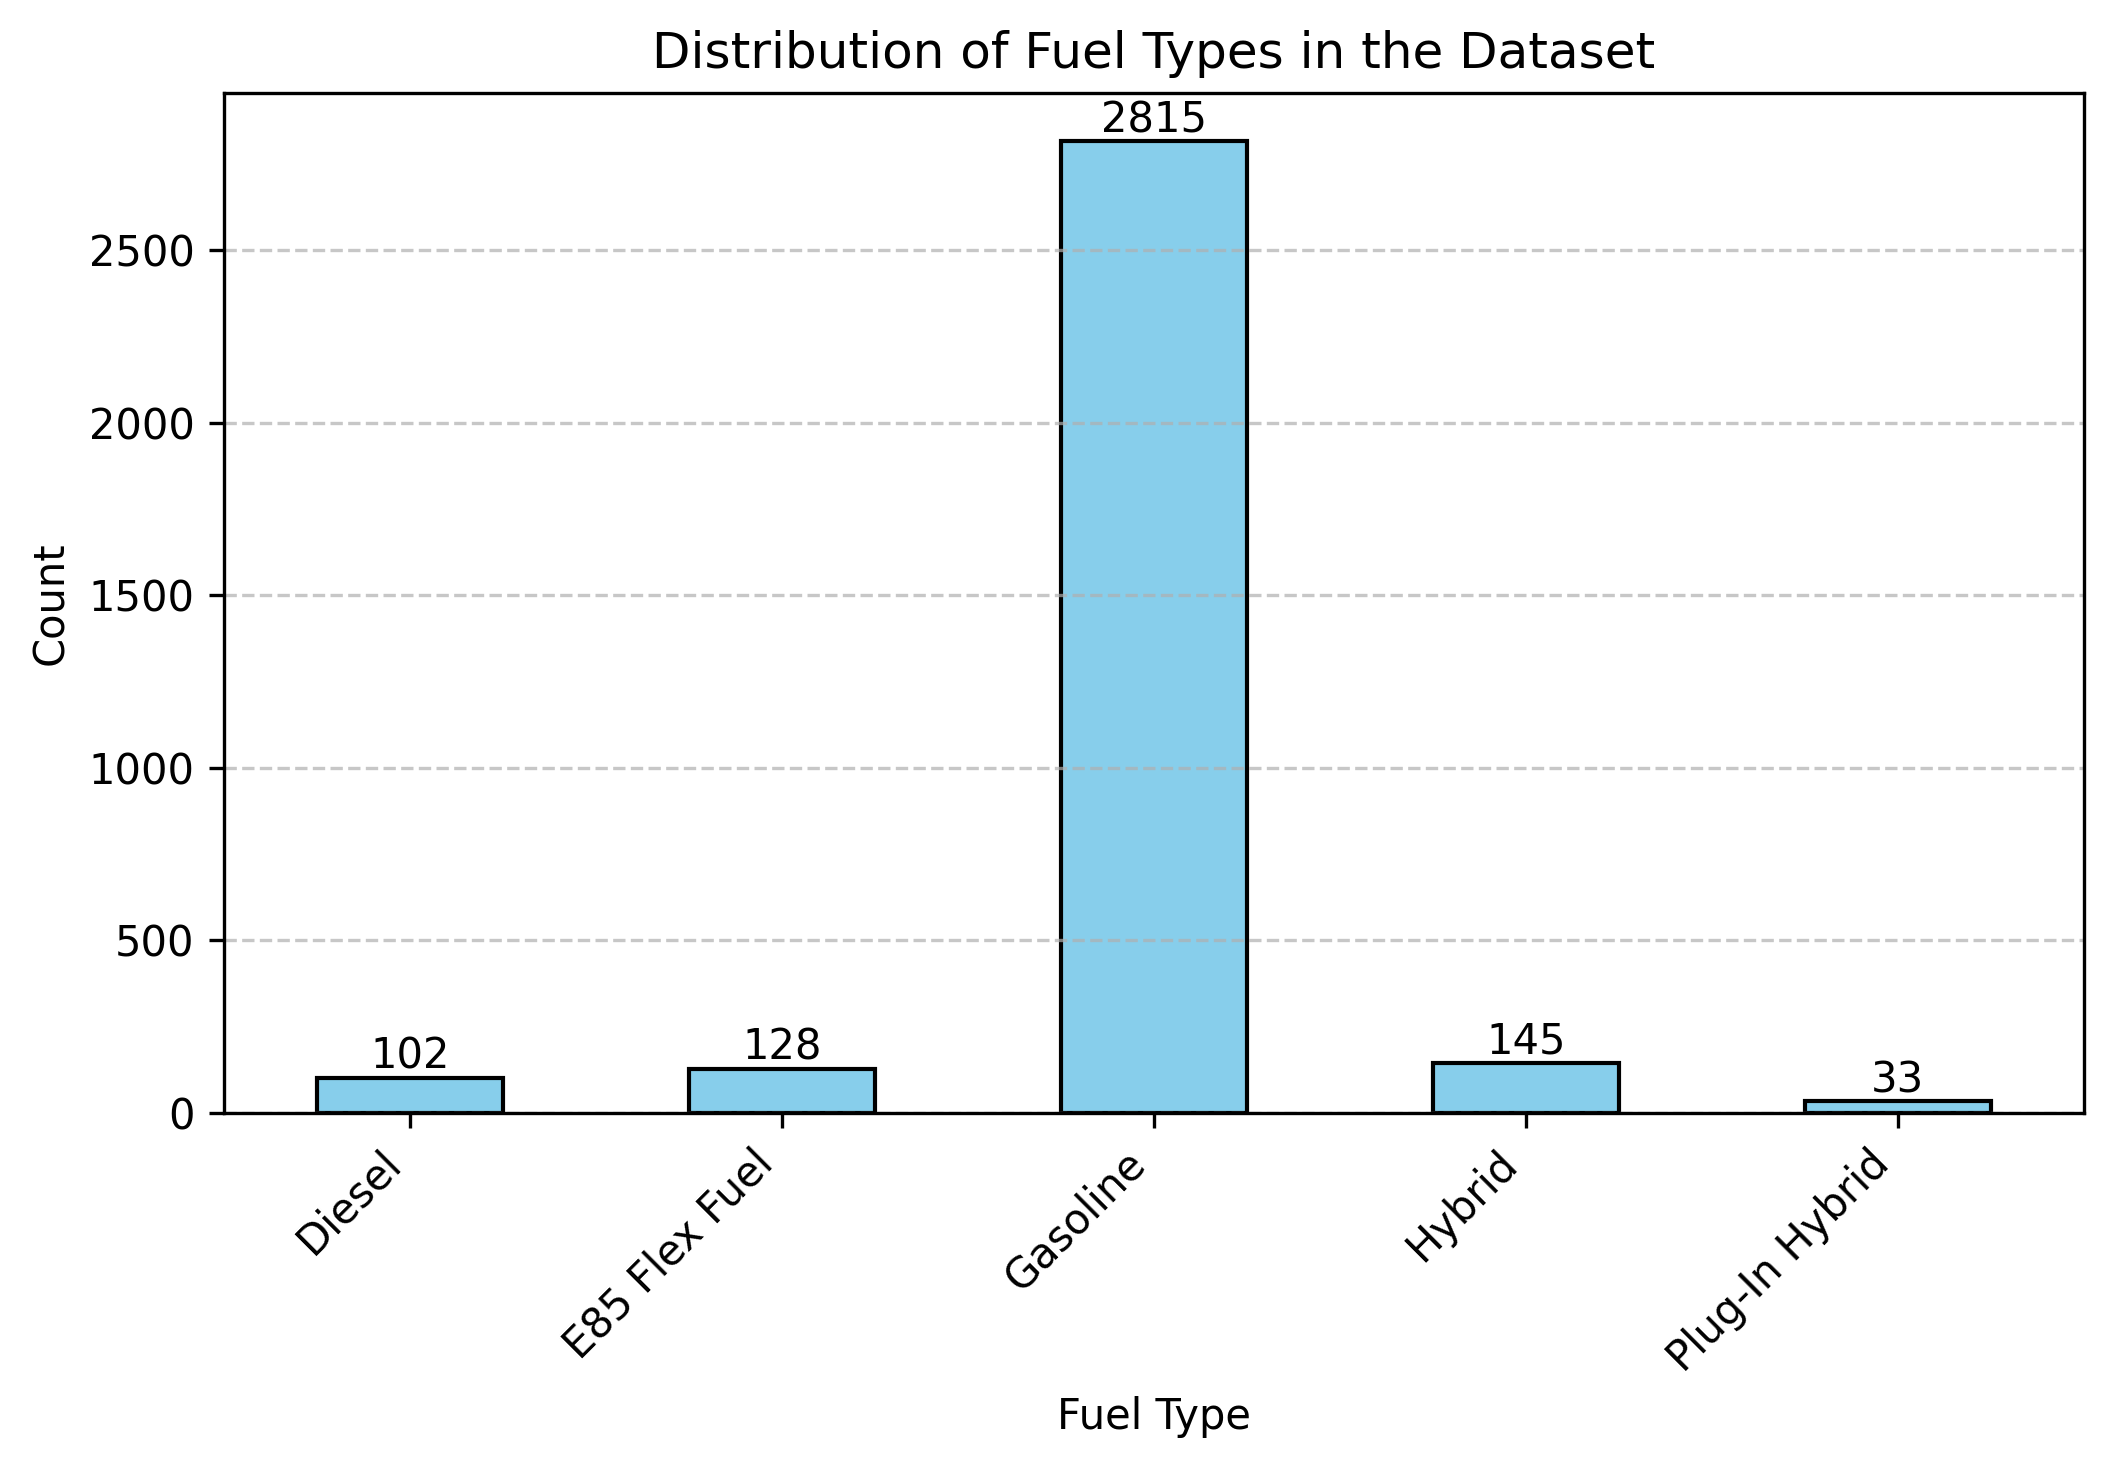
\includegraphics[width=\textwidth]{total_fuel.png}
        \caption{Distribution of car fuel type in the dataset}
        \label{fig:total_fuel}
    \end{minipage}\hfill
    \begin{minipage}{0.45\textwidth}
        \centering
        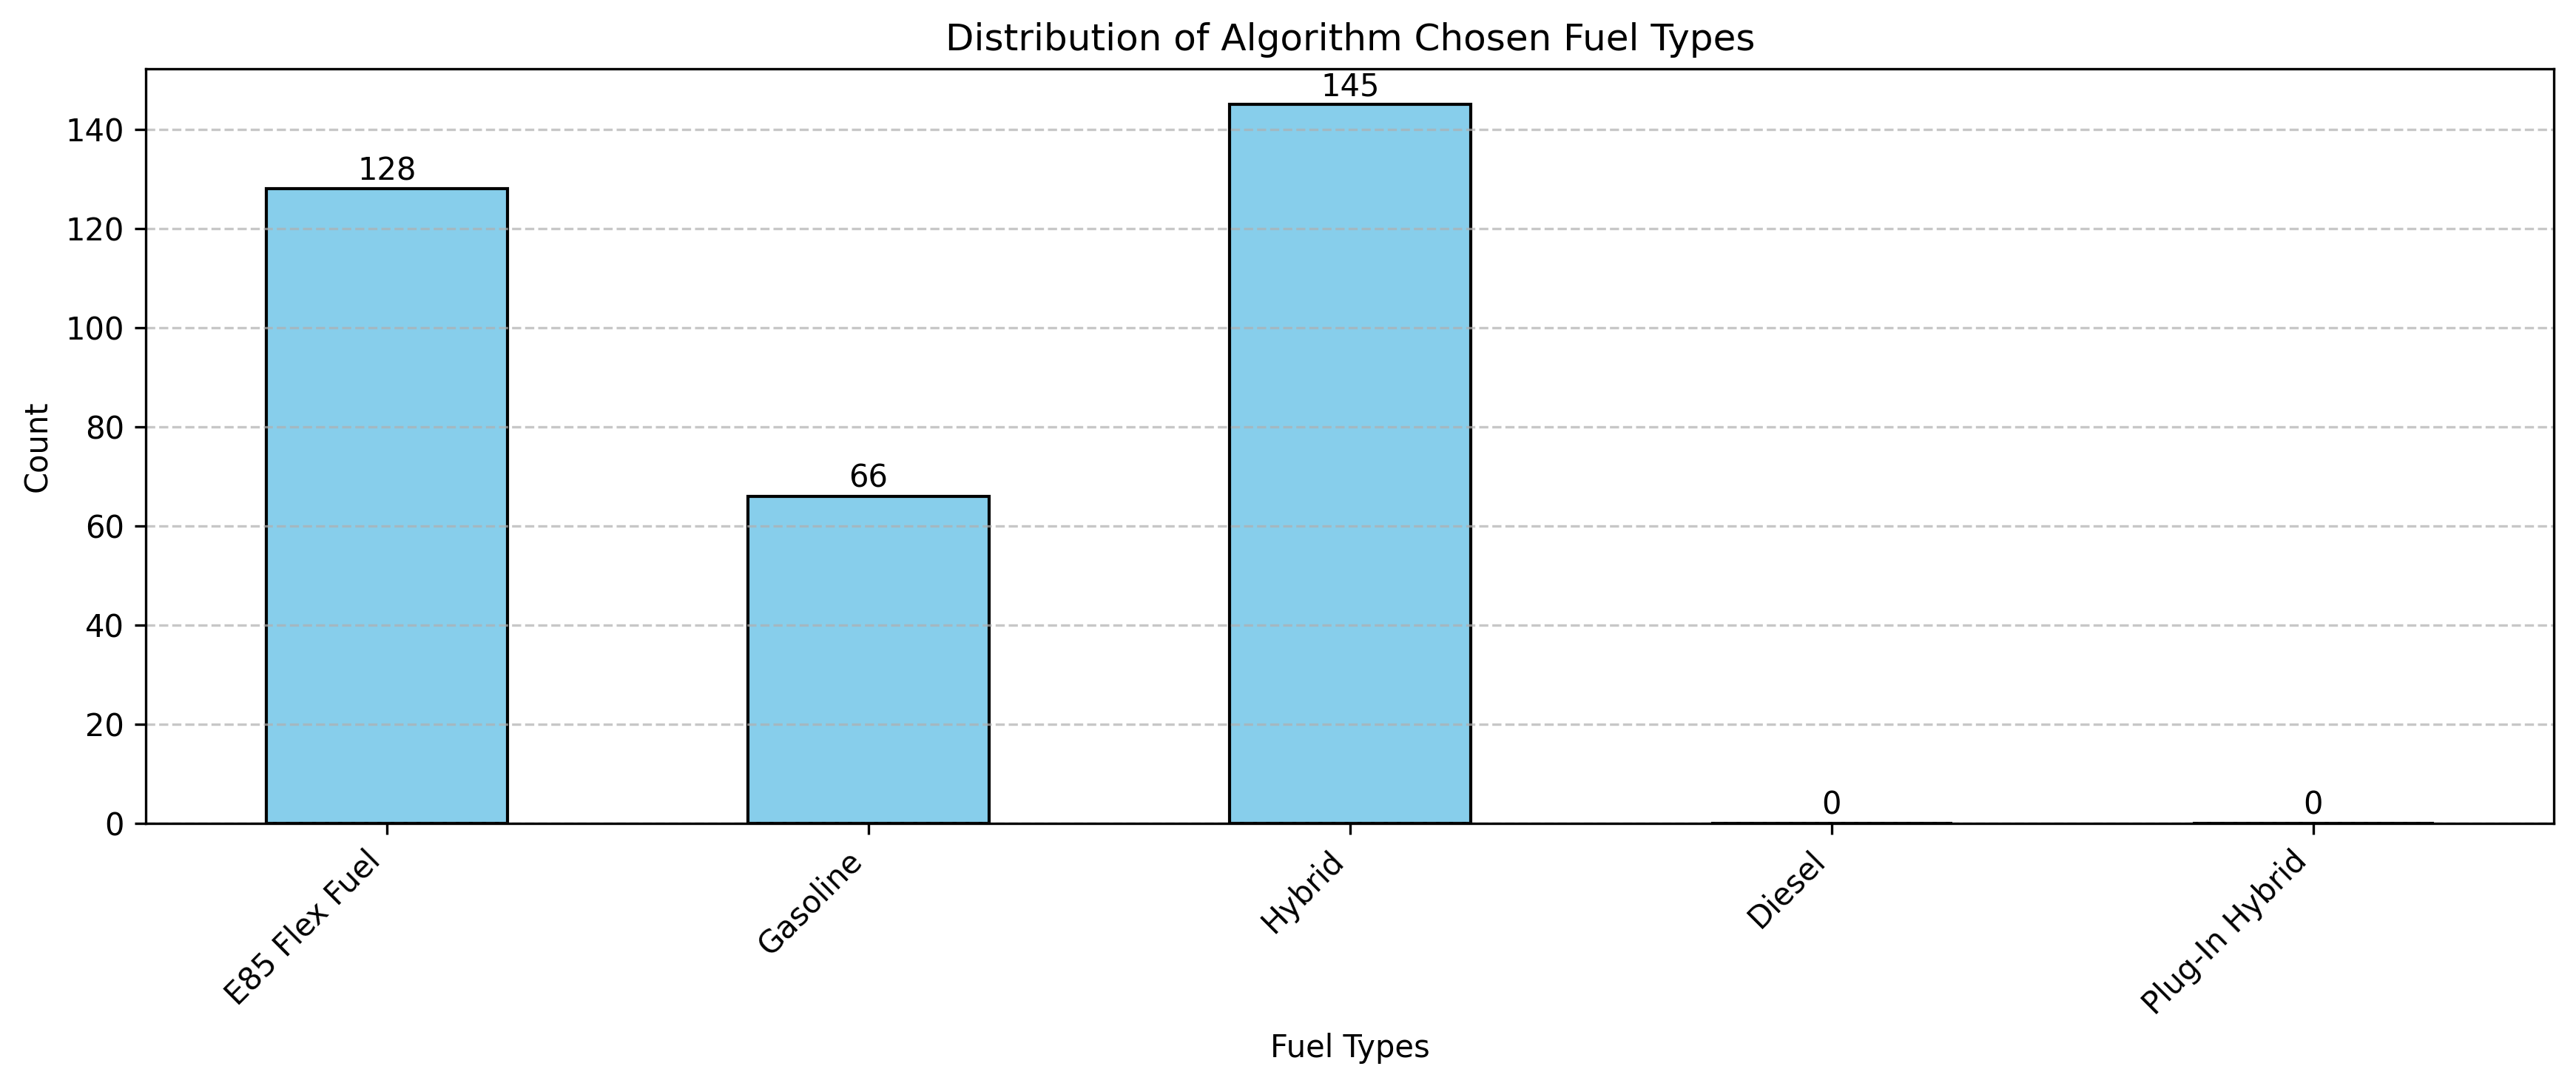
\includegraphics[width=\textwidth]{algo_fuel.png}
        \caption{Distribution of car fuel type from CVXPY}
        \label{fig:algo_fuel}
    \end{minipage}\hfill
    \begin{minipage}{0.45\textwidth}
        \centering
        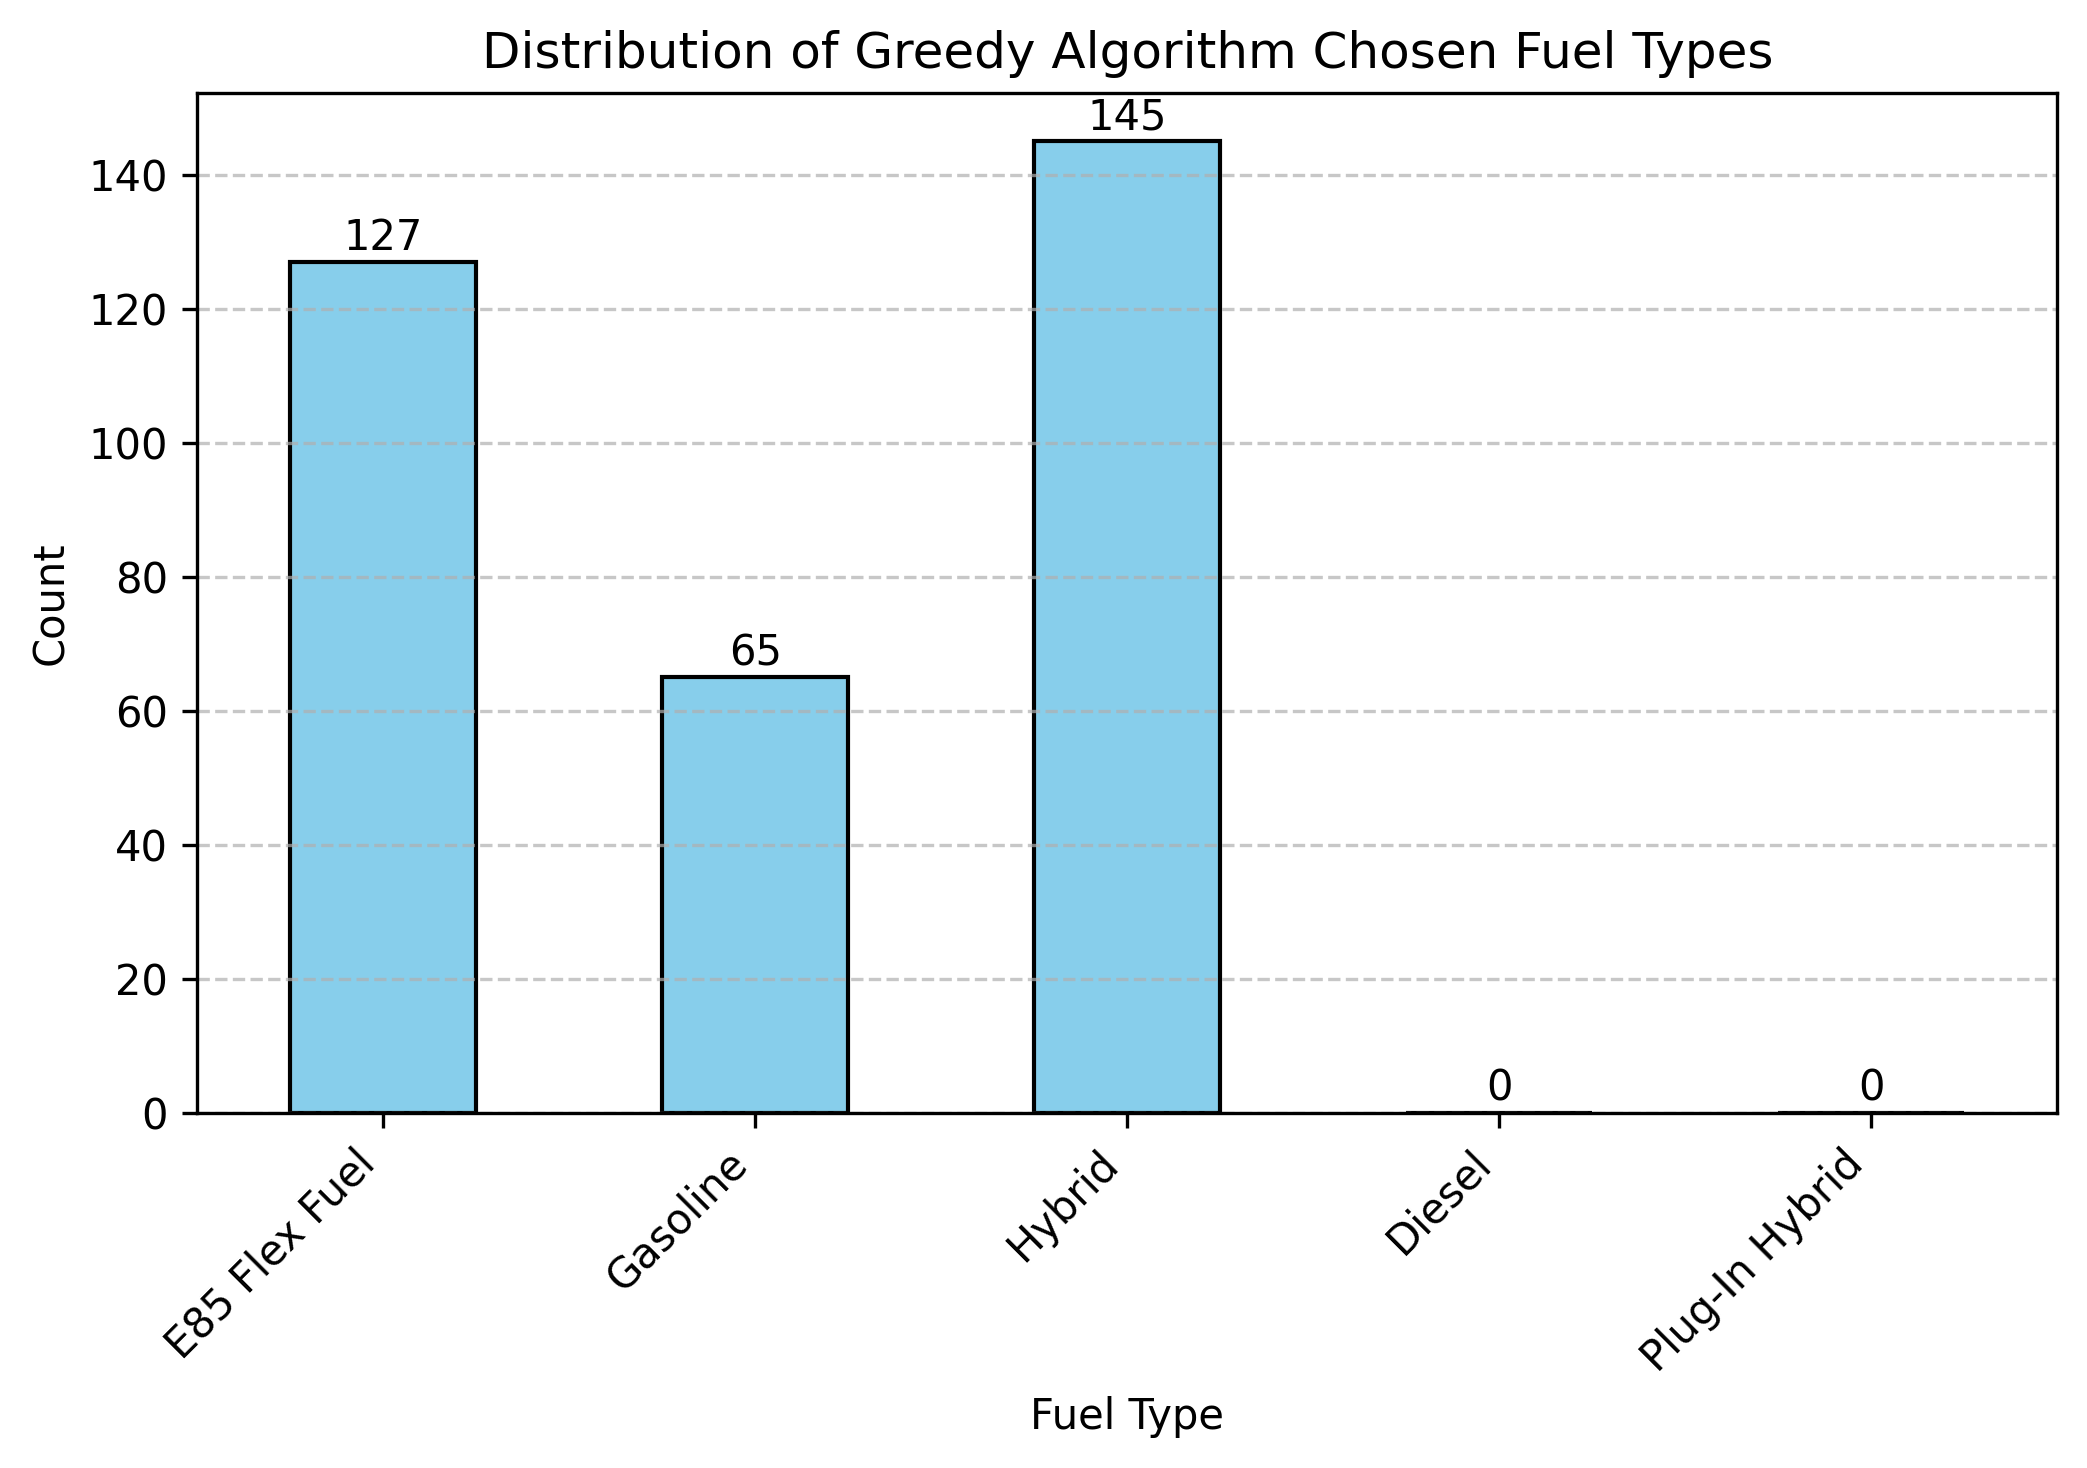
\includegraphics[width=\textwidth]{greedy_budget_fuel.png}
        \caption{Distribution of car fuel type from Budget Algorithm}
        \label{fig:greedy_budget_fuel}
    \end{minipage}\hfill
    \begin{minipage}{0.45\textwidth}
        \centering
        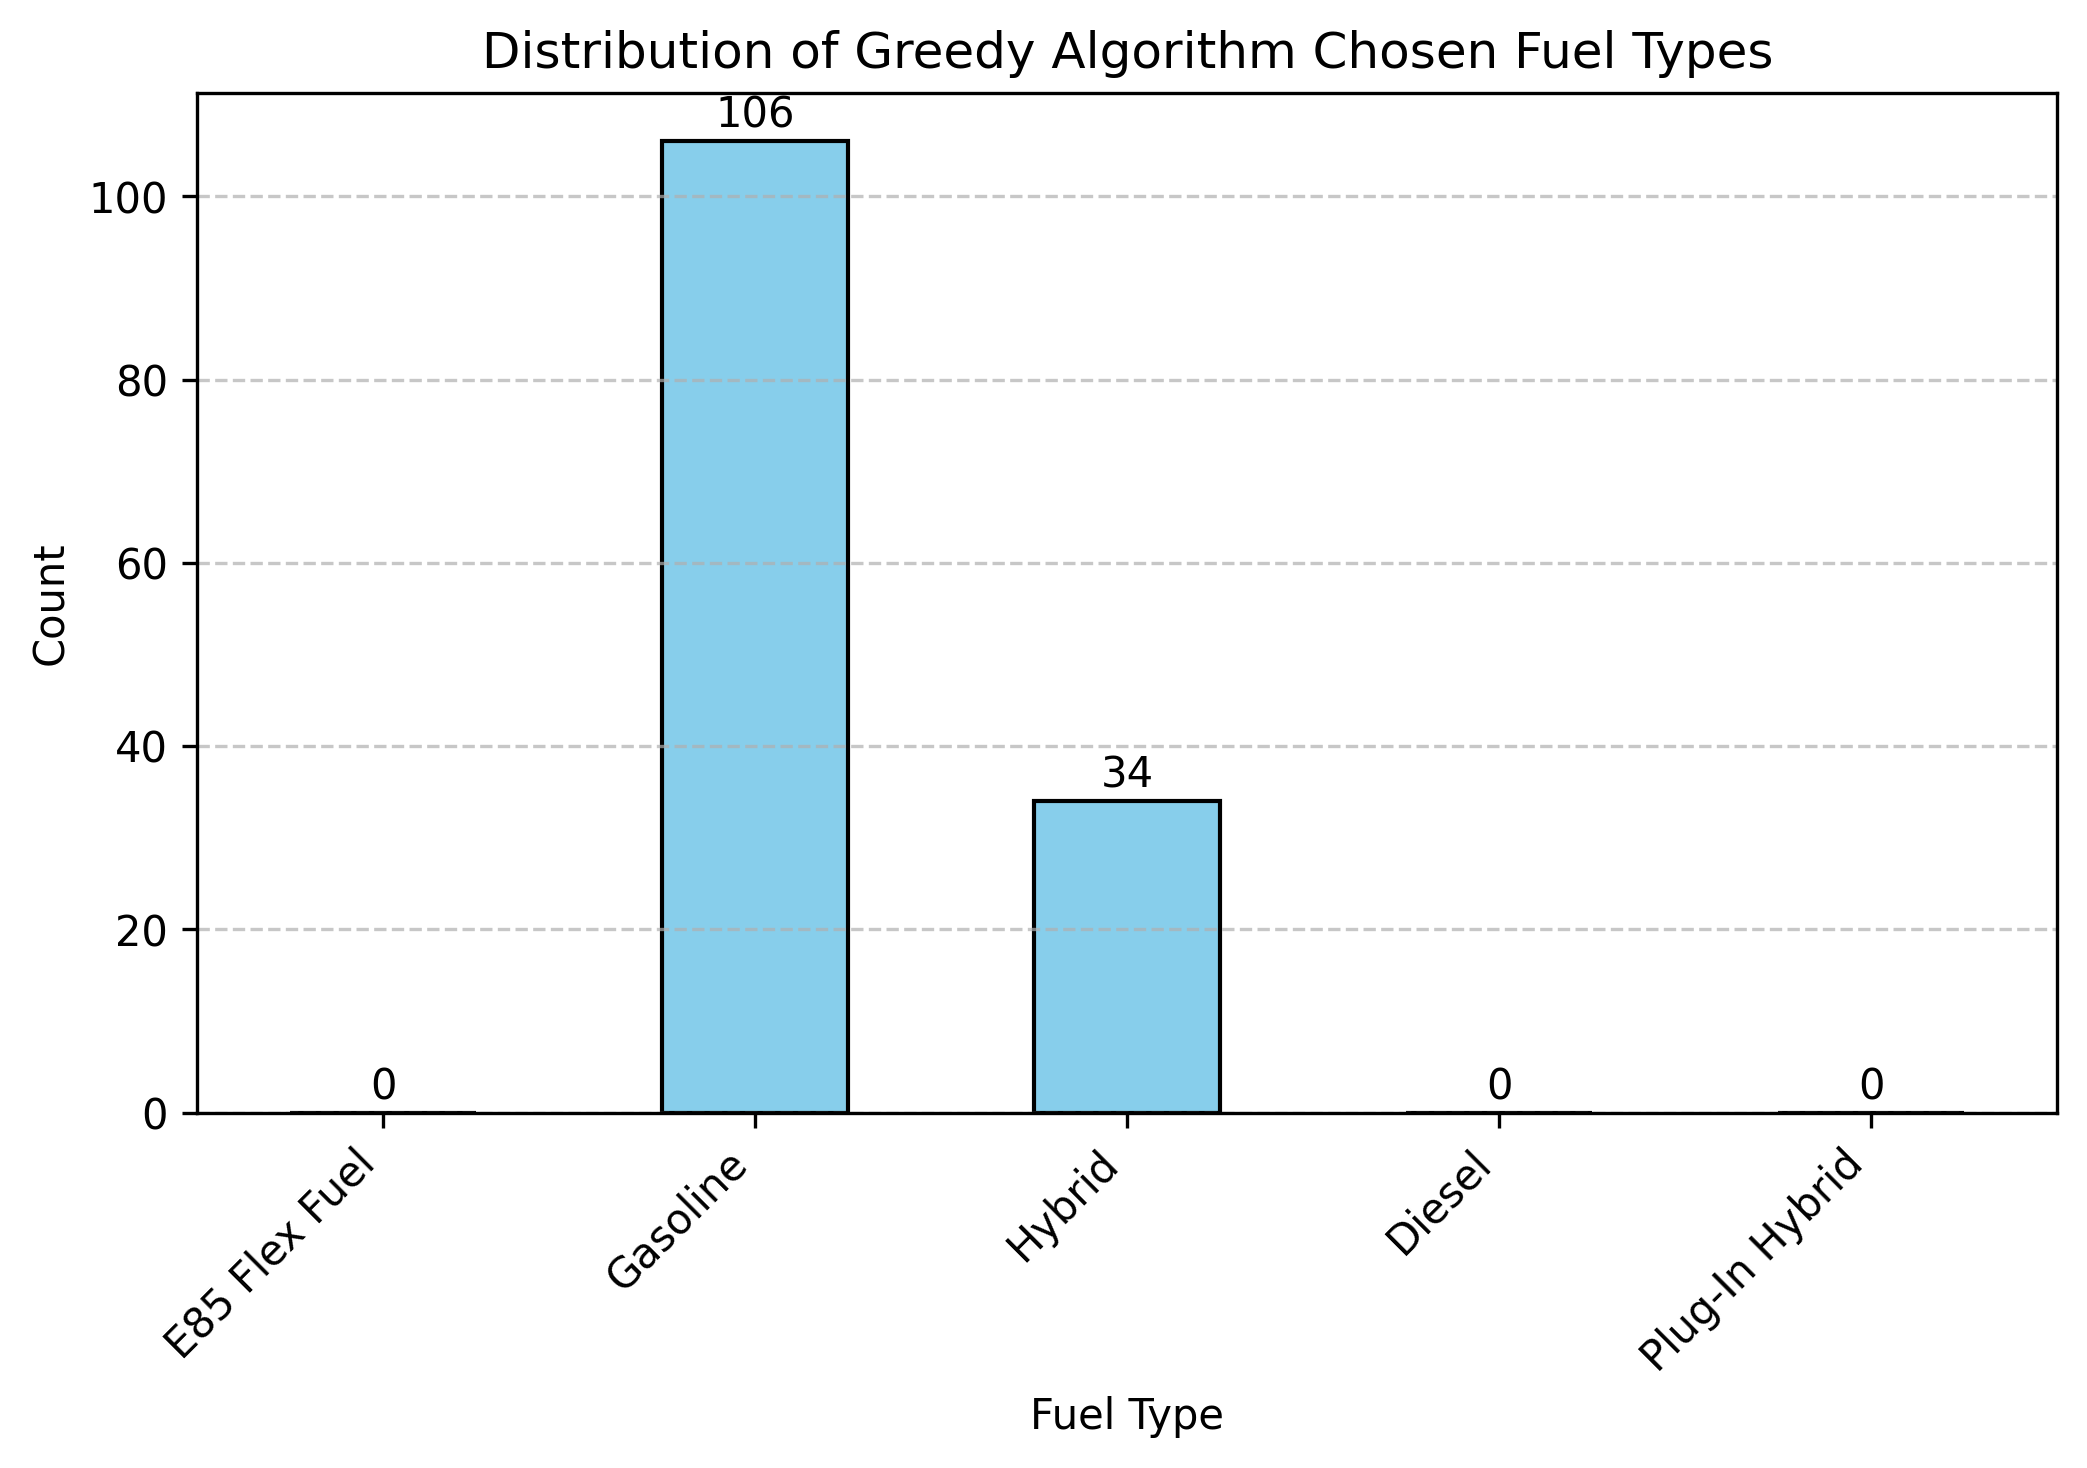
\includegraphics[width=\textwidth]{greedy_size_fuel.png}
        \caption{Distribution of car fuel type from Size Algorithm}
        \label{fig:greedy_size_fuel}
    \end{minipage}
\end{figure}
\subsubsection{Compare Selection on Import/Domestic Cars}
A similar data analysis was conducted on imported versus domestic cars. The histograms below show import types of the dataset and selected cars from all three algorithms. \par On average, imported cars generate less profit than domestic cars. In the dataset, domestic cars composes 52$\%$ of the total available cars. Both CVXPY method and Budget Algorithm's selection are composed of $70\%$ domestic cars, and the number of domestic cars from Size Algorithm's choice takes up $64\%$ percent of the total cars: In general, the histograms reflect that they all capture this trend and incorporate it into their strategies. This suggests that both algorithms are aware of the profitability difference between imported and domestic cars, yet the way they weigh this factor may differ based on their optimization approaches.
\begin{figure}[h]
    \centering
    \begin{minipage}{0.45\textwidth}
        \centering
        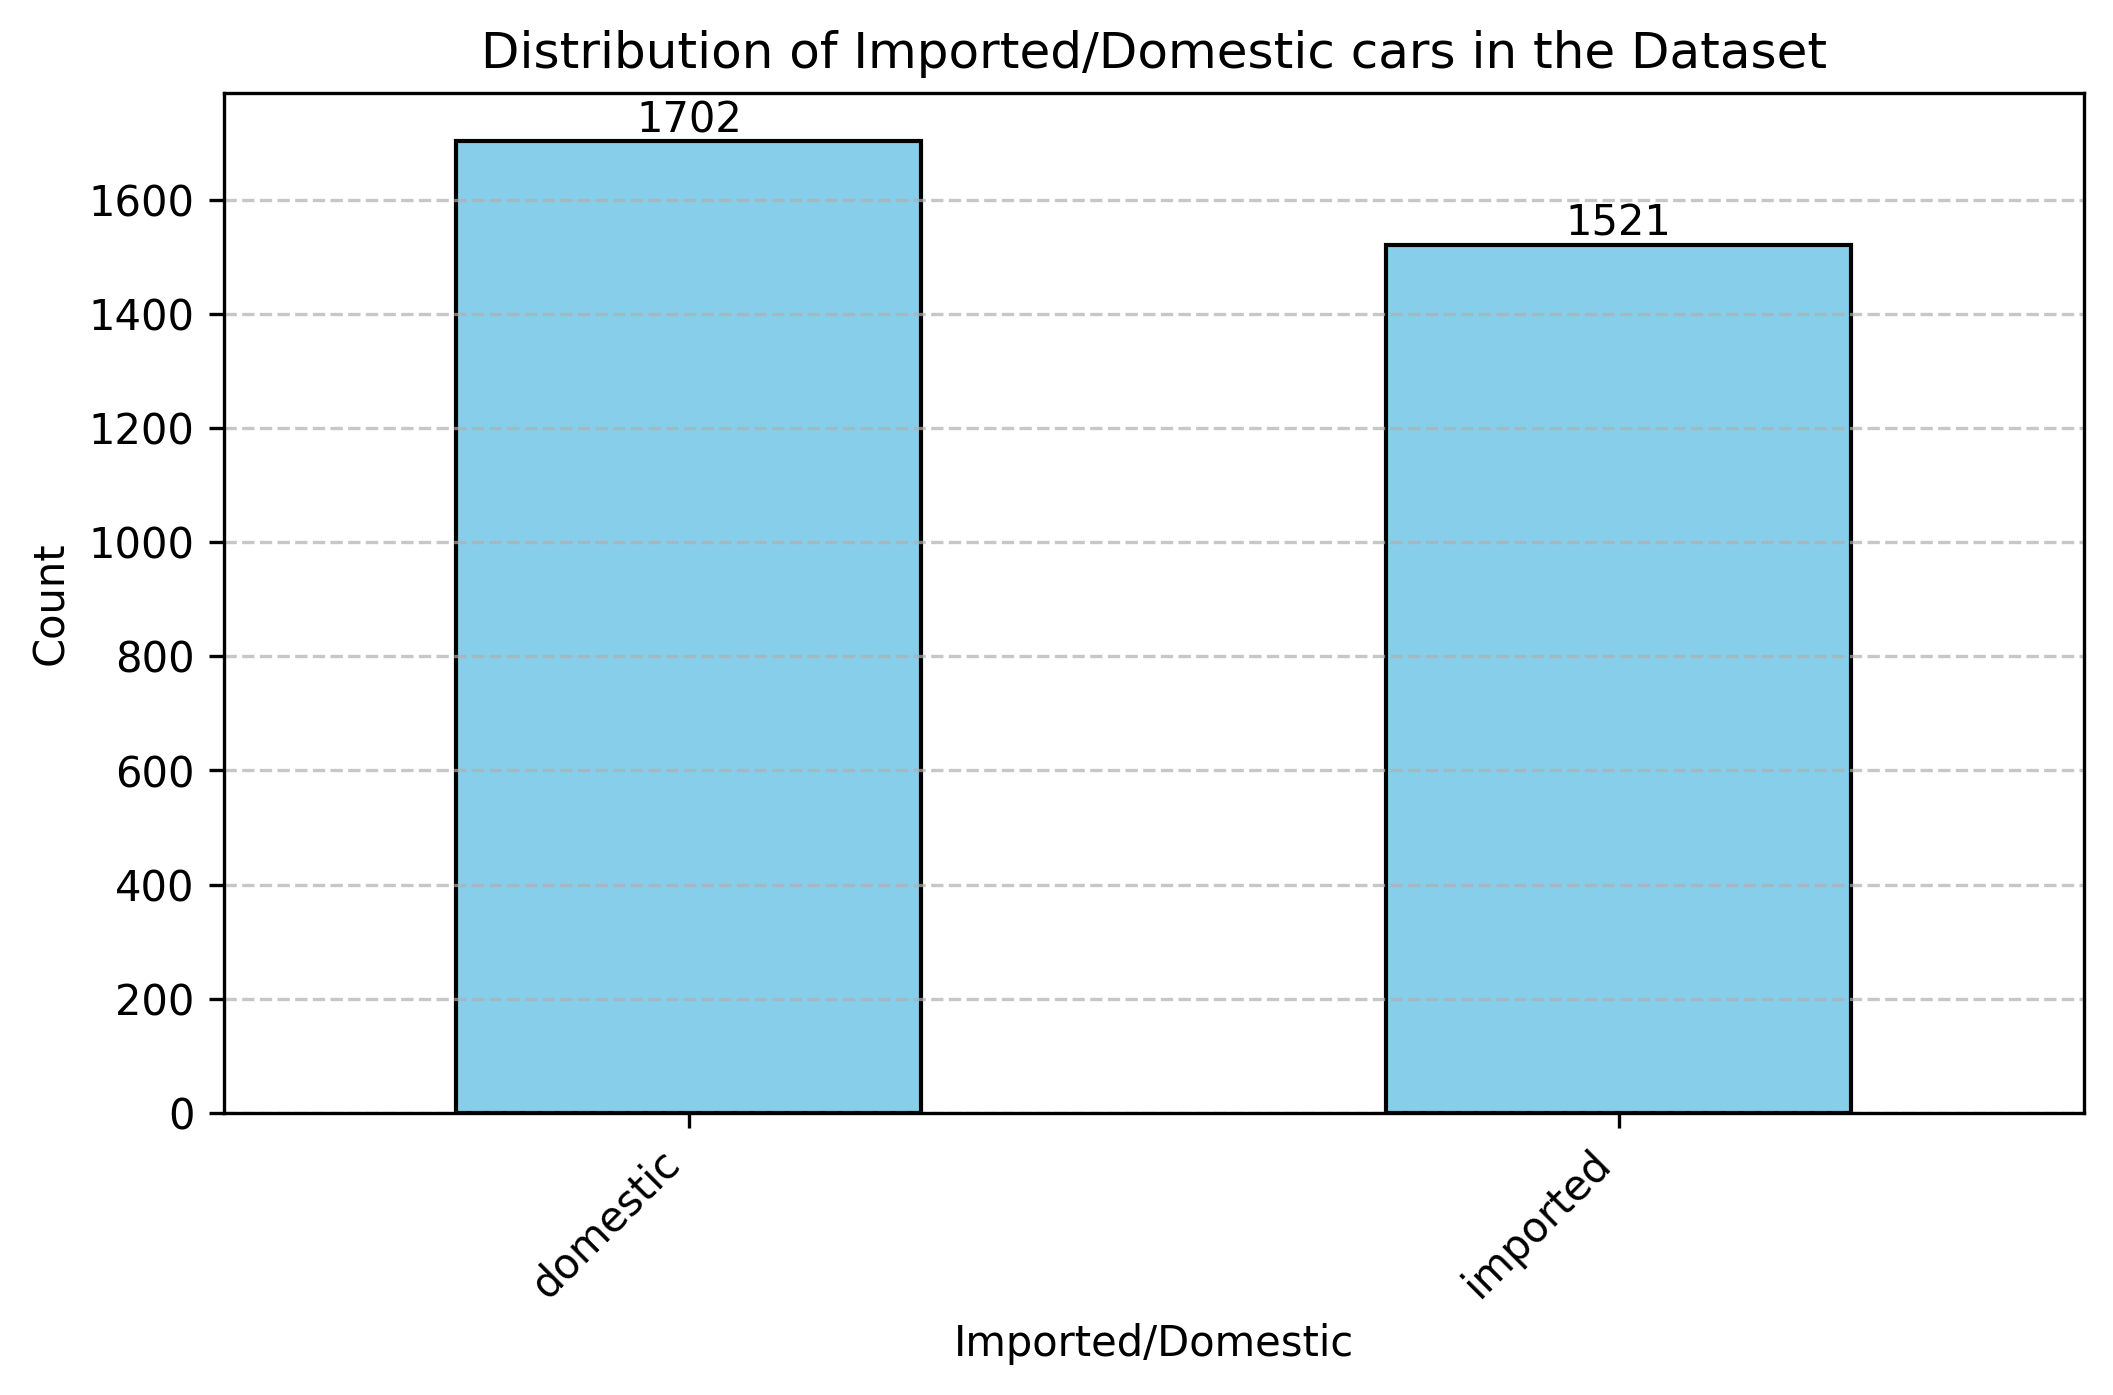
\includegraphics[width=\textwidth]{total_import.png}
        \caption{Distribution of car import condition in the dataset}
        \label{fig:total_import}
    \end{minipage}\hfill
    \begin{minipage}{0.45\textwidth}
        \centering
        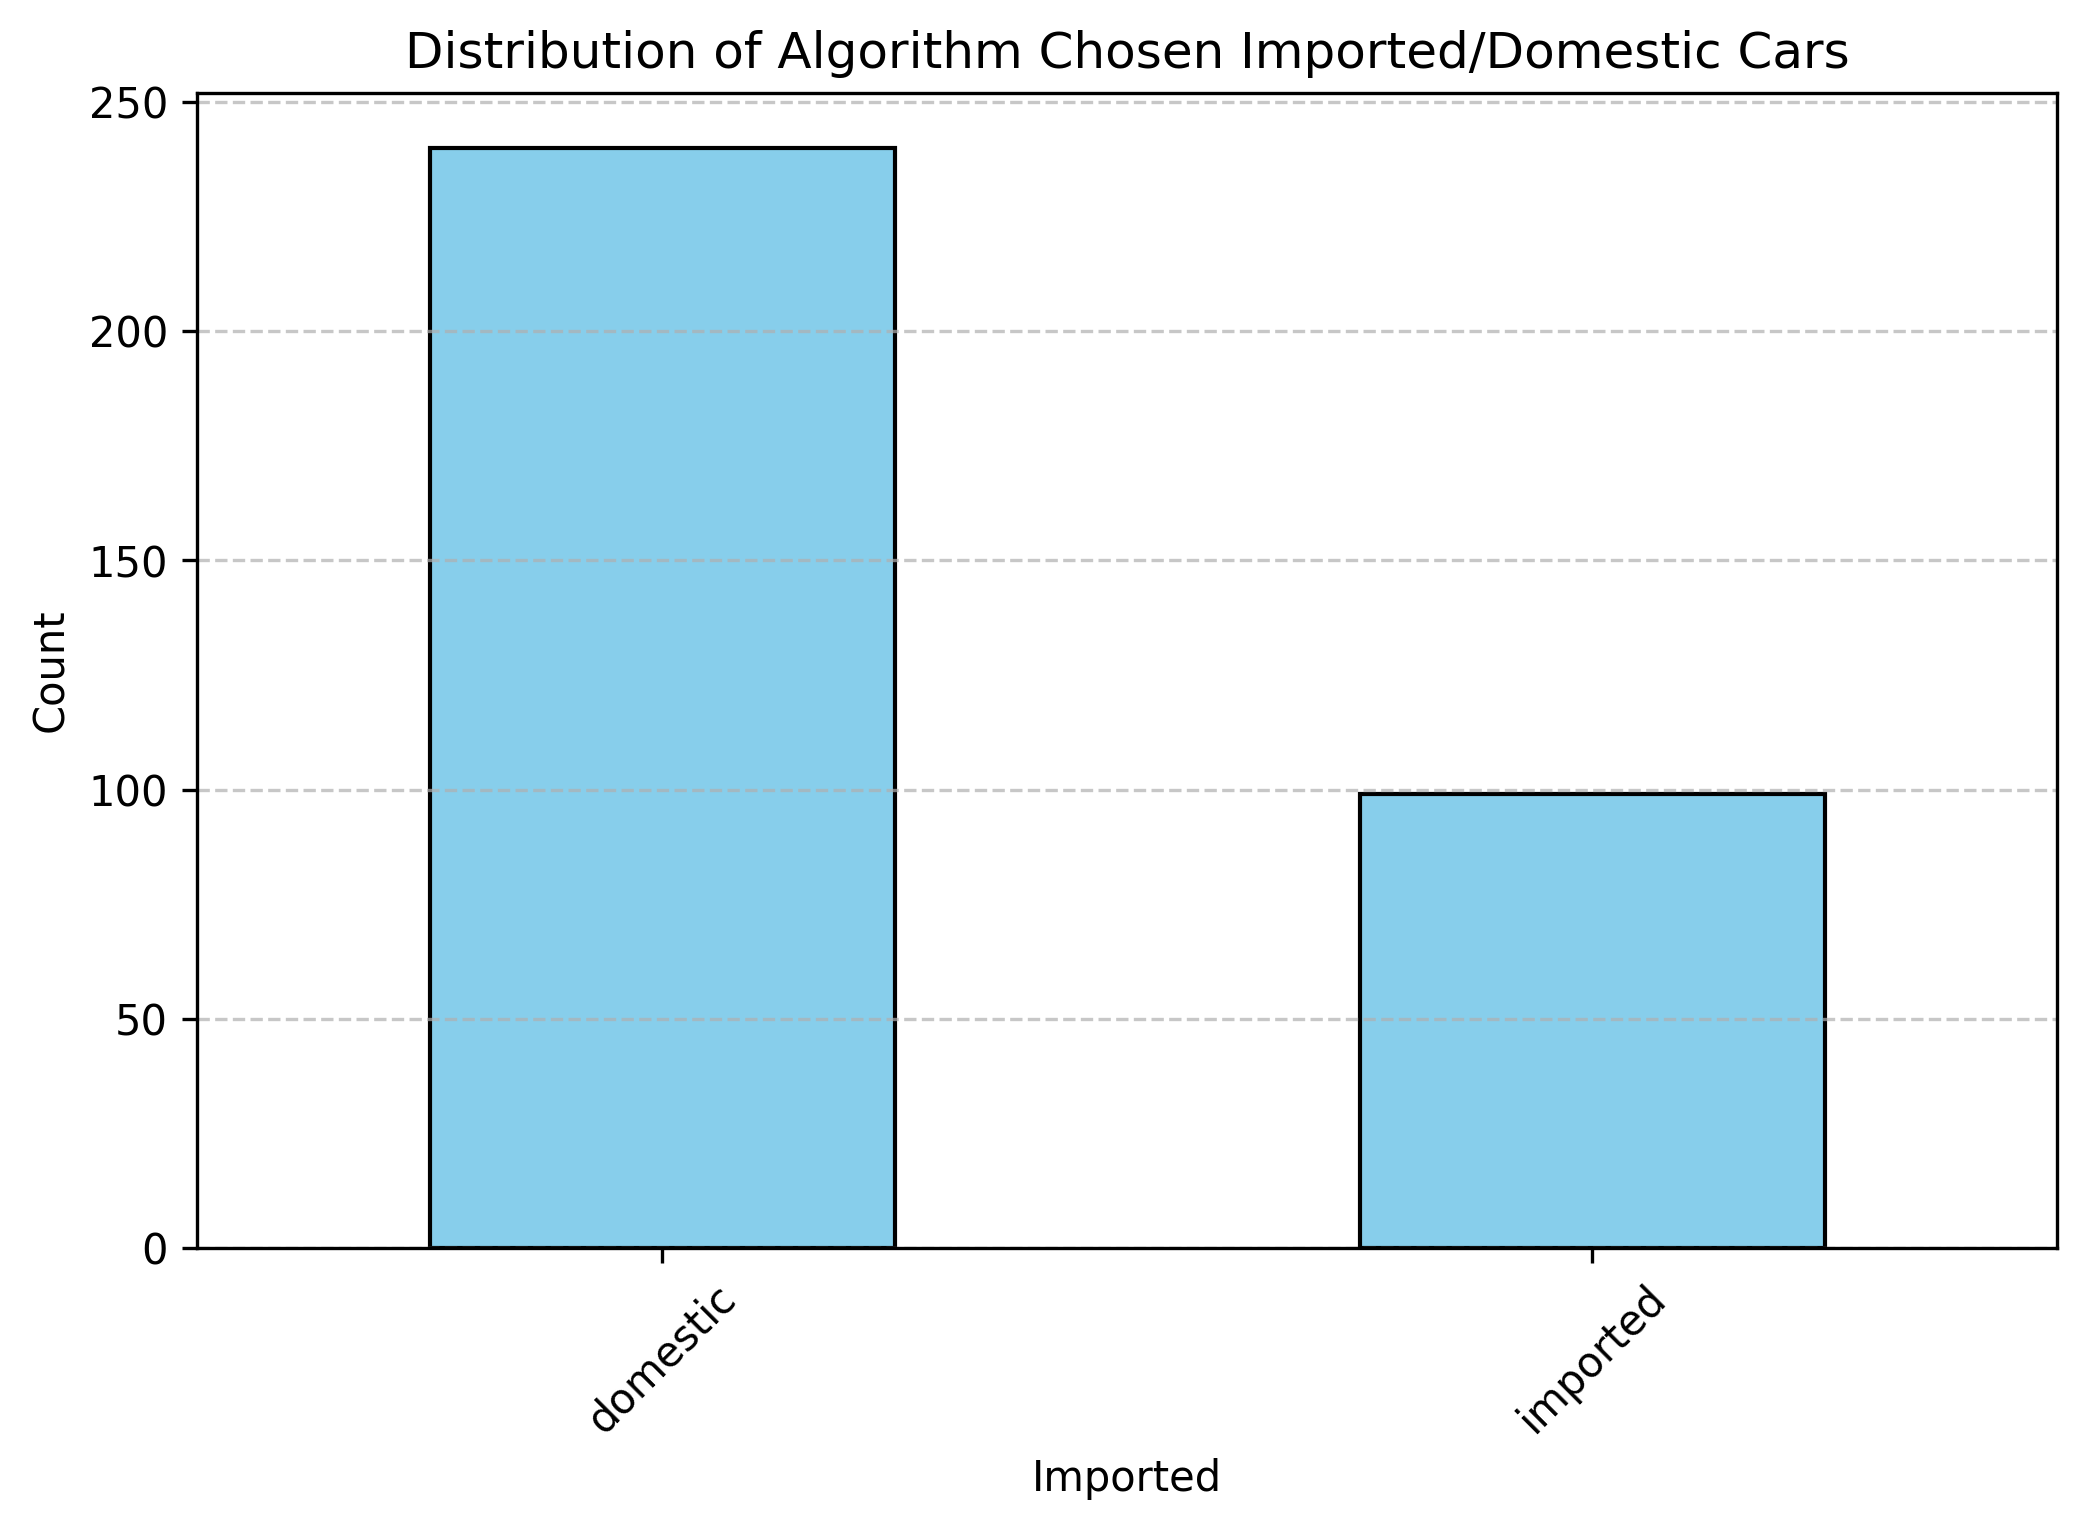
\includegraphics[width=\textwidth]{algo_import.png}
        \caption{Distribution of car import condition from CVXPY}
        \label{fig:algo_import}
    \end{minipage}\hfill
    \begin{minipage}{0.45\textwidth}
        \centering
        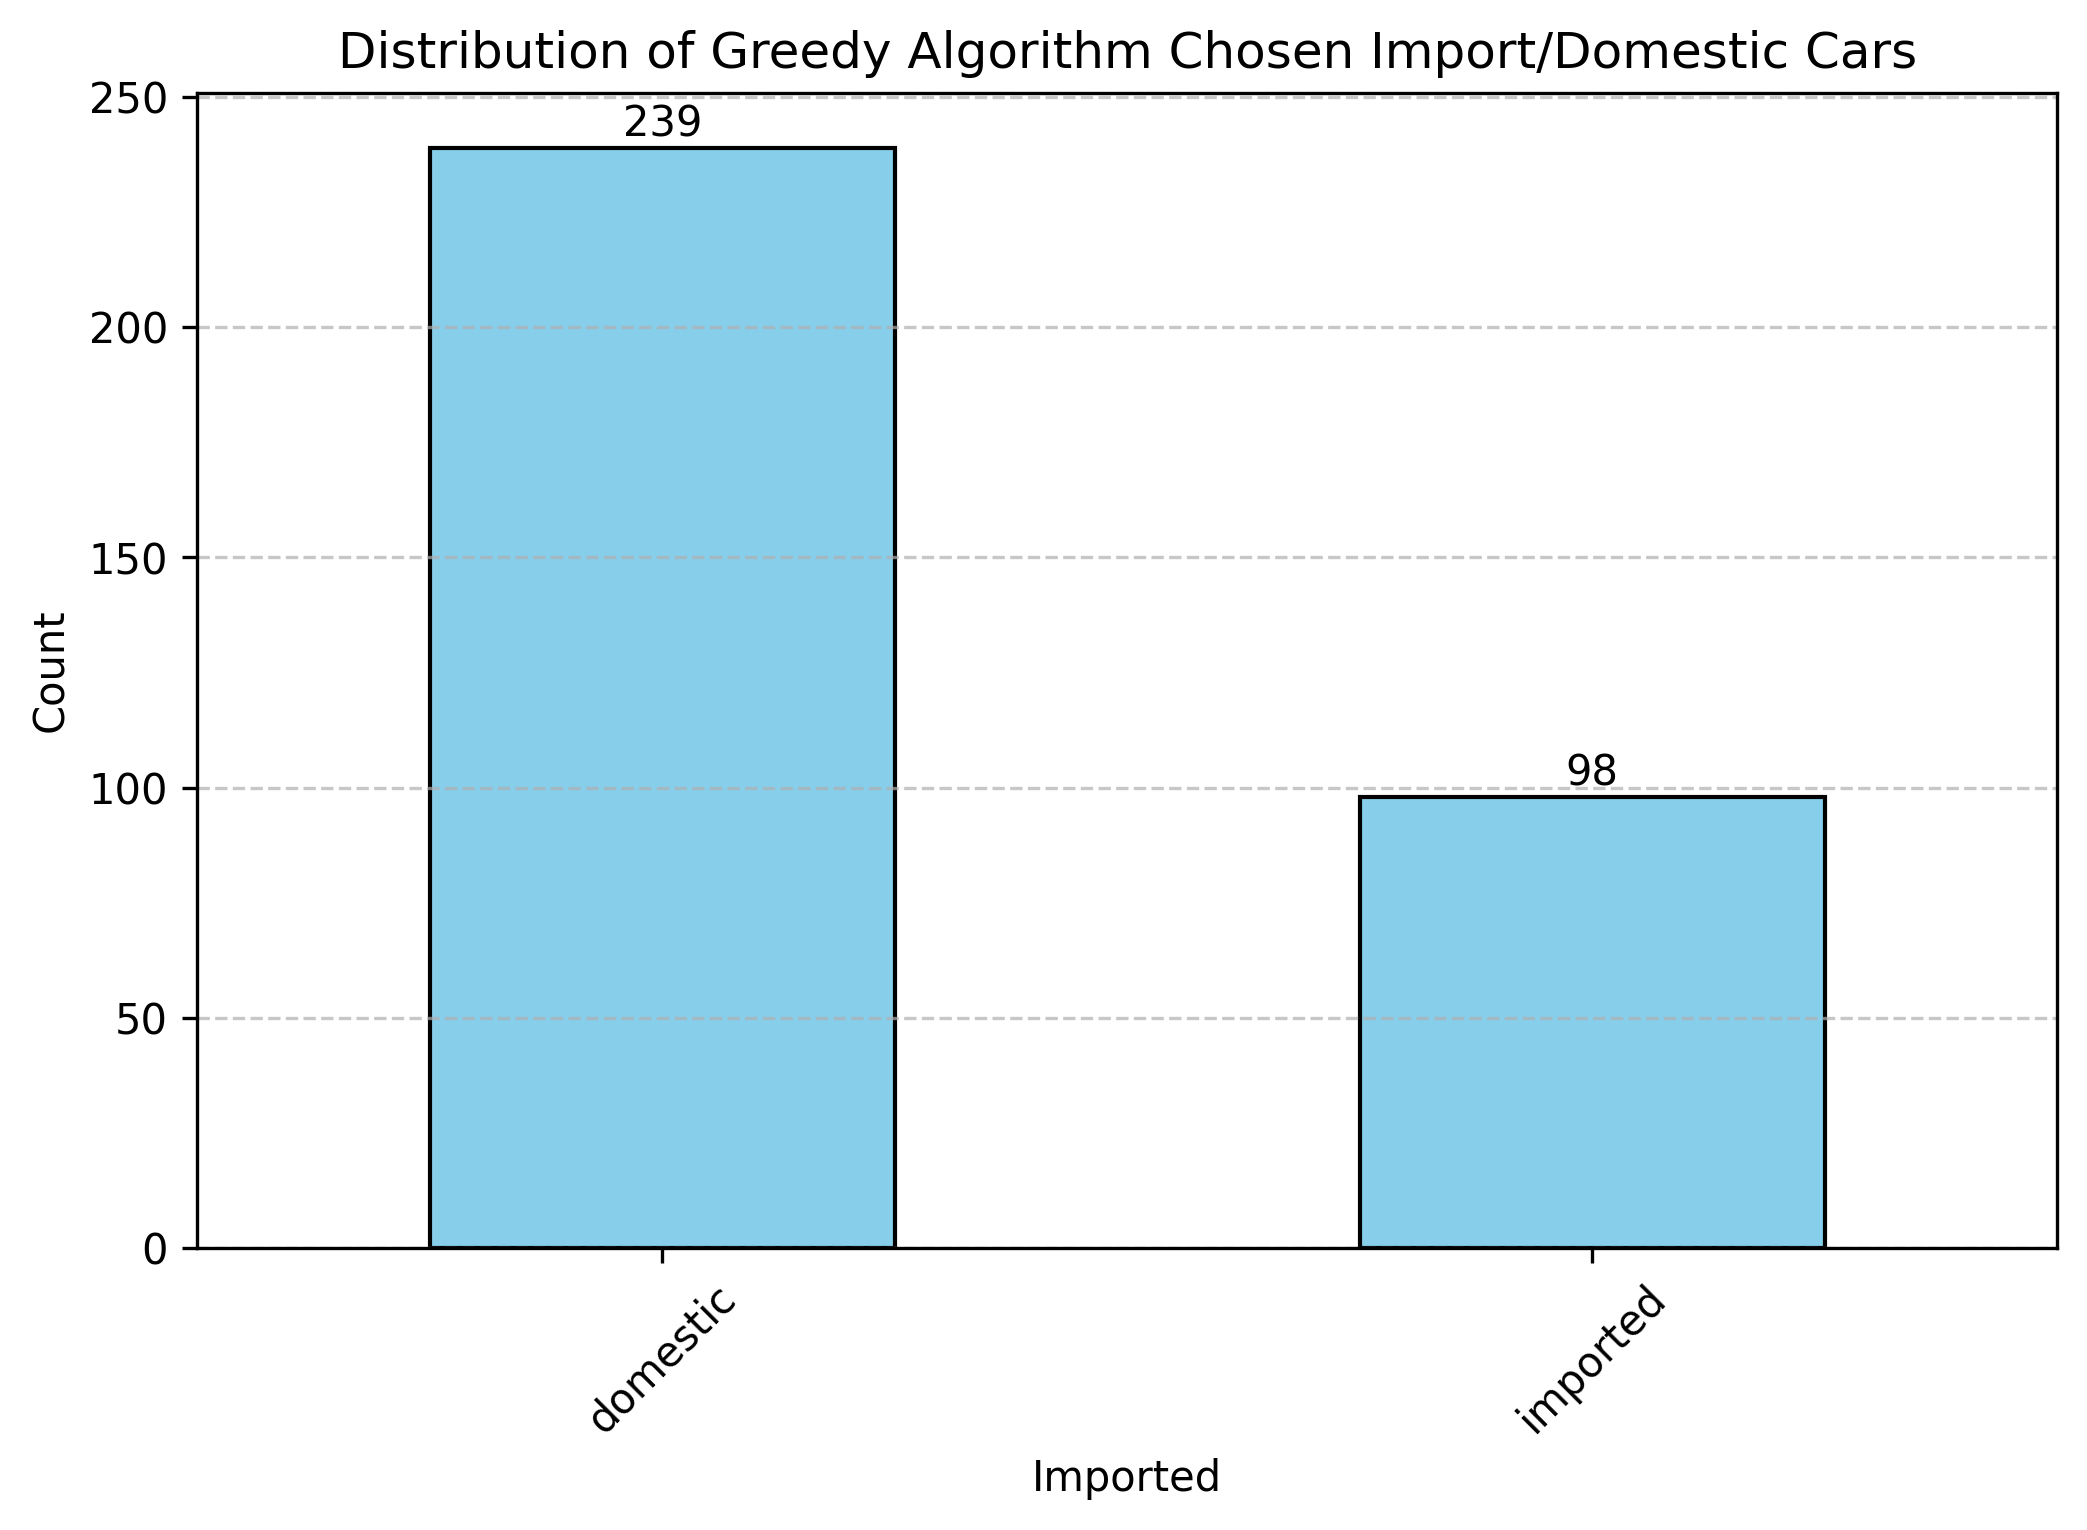
\includegraphics[width=\textwidth]{greedy_budget_import.png}
        \caption{Distribution of car import condition from Budget Algorithm}
        \label{fig:greedy_budget_import}
    \end{minipage}\hfill
    \begin{minipage}{0.45\textwidth}
        \centering
        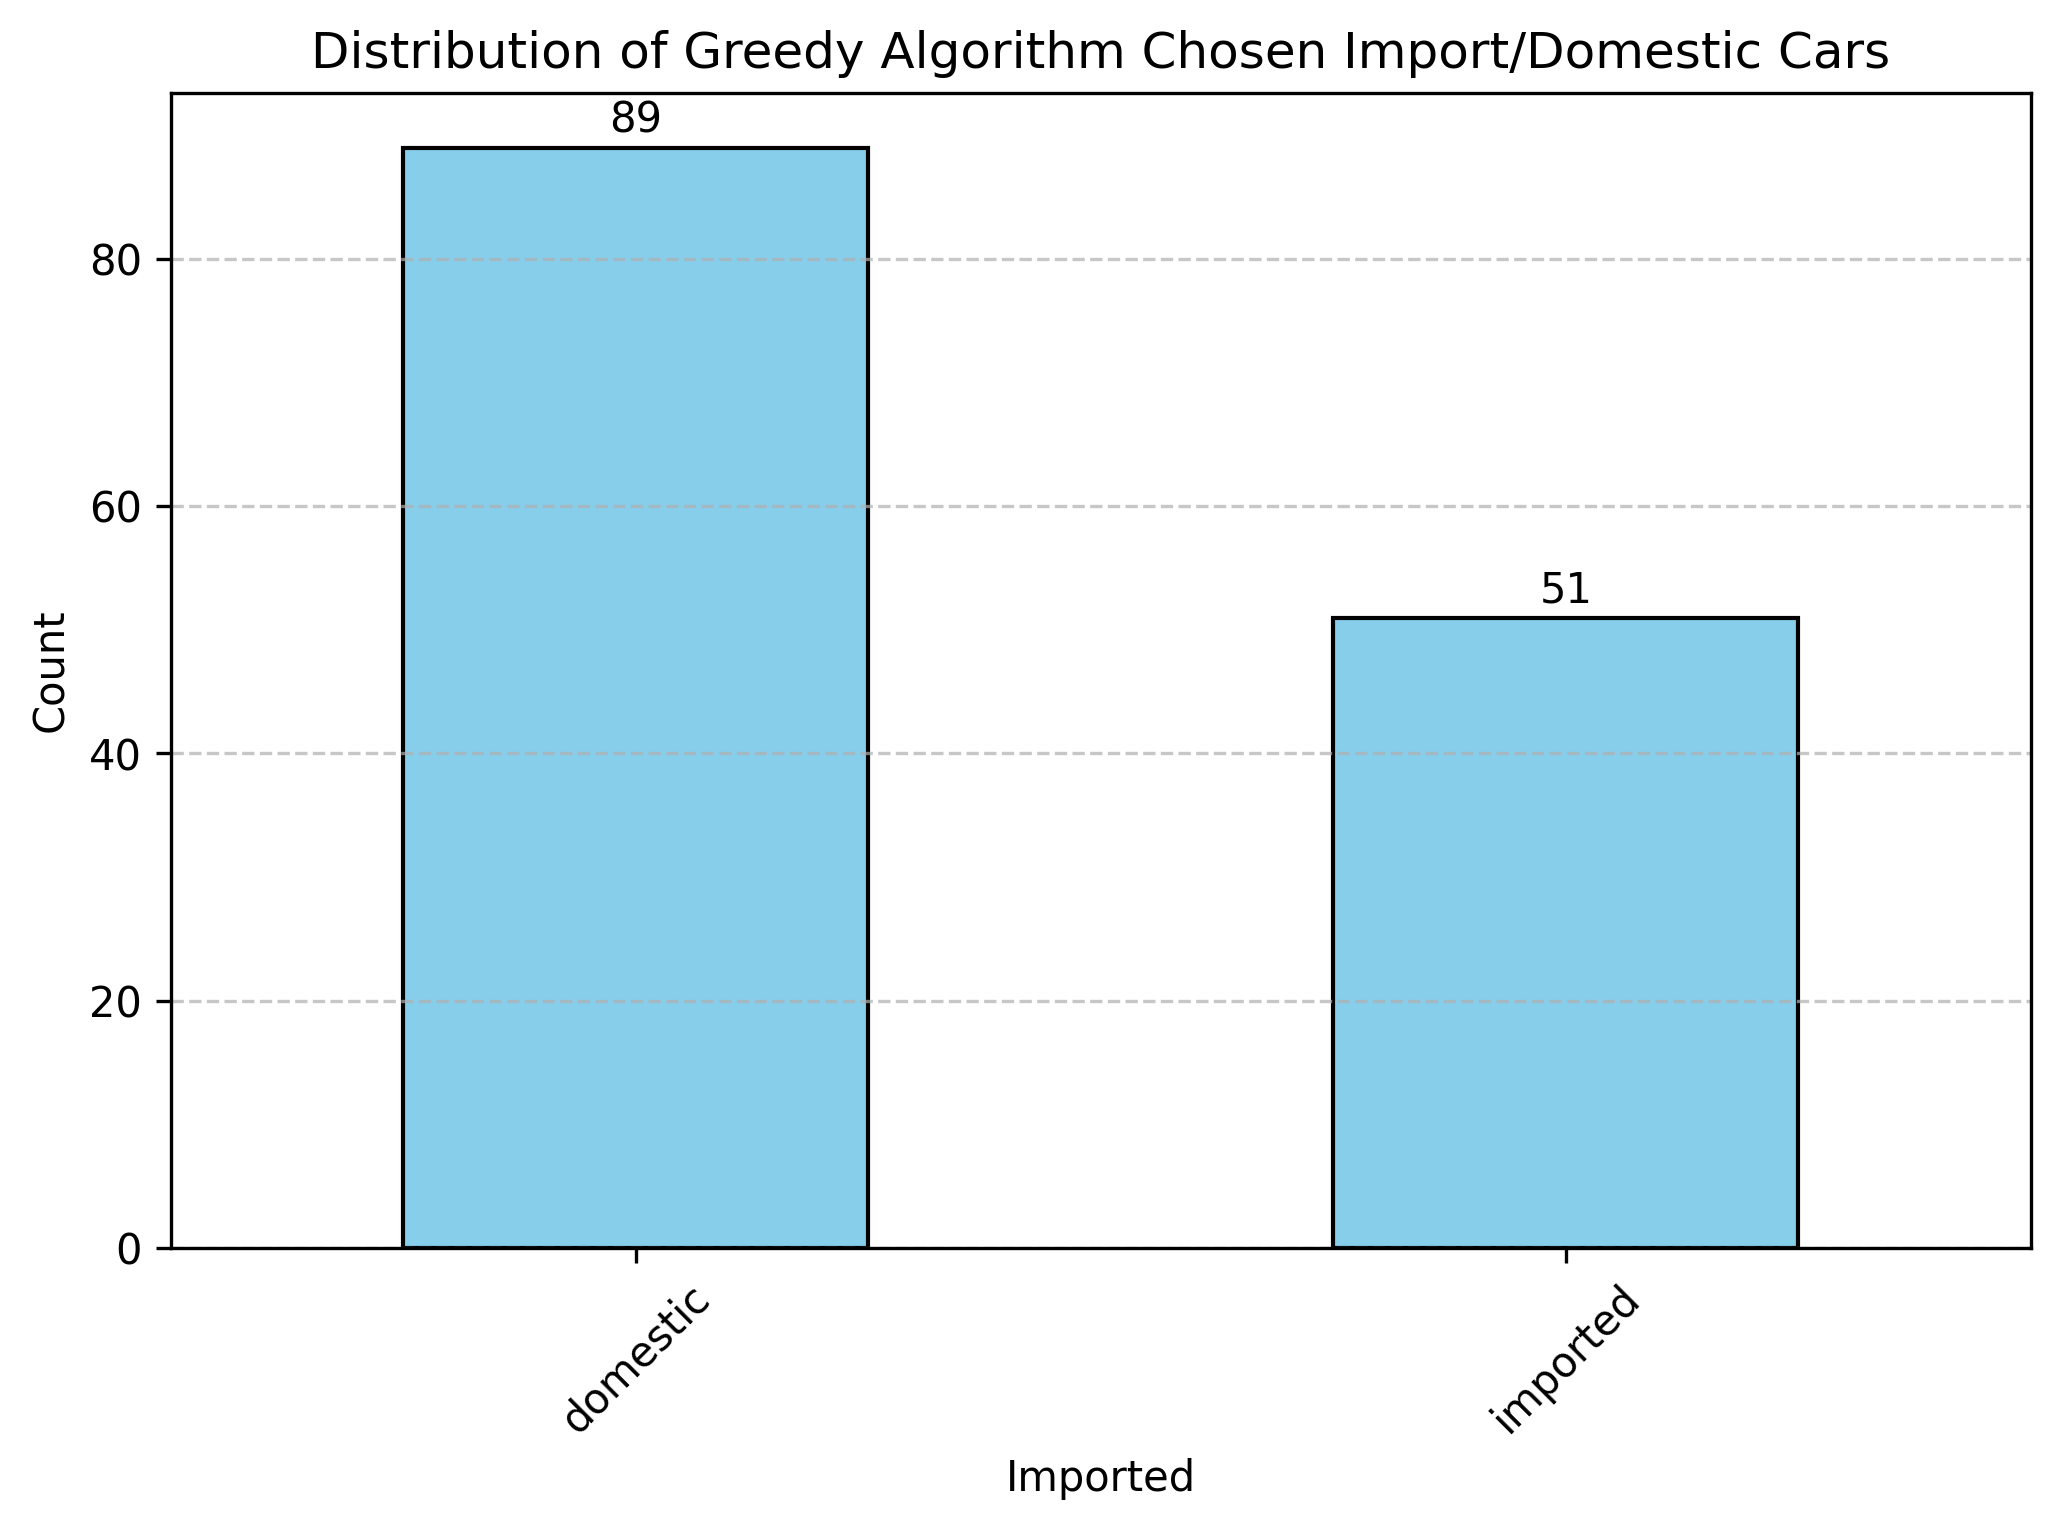
\includegraphics[width=\textwidth]{greedy_size_import.png}
        \caption{Distribution of car import condition from Size Algorithm}
        \label{fig:greedy_size_import}
    \end{minipage}
\end{figure}
\subsubsection{Compare Brand Selection between Algorithms}
From the previous two analysis, we noticed that the output from CVXPY and Budget Algorithm is amazingly similar. Therefore, a further exploration on the car brand selection is made to research their performance. \par
In the histogram shown below, it is obvious that the CVXPY and Budget Algorithm yet again present similar results, where the Budget Algorithm omits one Ford car and one Aston car. This similarity, combined with similarities in terms of cars sold, total profit amount, fuel type selection and import/dometic car selection, suggests that Budget Algorithm is a better approximation than Size Algorithm.\par
Comparing the distribution of car brands from the CVXPY algorithm and the Size Algorithm, we observe that the optimization solution proposed by the greedy algorithm includes significantly fewer brands than the CVXPY solution: the greedy algorithm selects only 19 different brands, whereas CVXPY includes 34 brands. Although the number of brands included by each algorithm may not directly reflect performance, a more diverse selection of brands can lead to a broader market appeal and potentially higher sales. This increased diversity suggests that CVXPY explores a wider range of options, allowing for a more balanced and optimized solution that accounts for various factors beyond immediate profit.\par
\begin{figure}[h]
    \centering
    \begin{minipage}{0.45\textwidth}
        \centering
        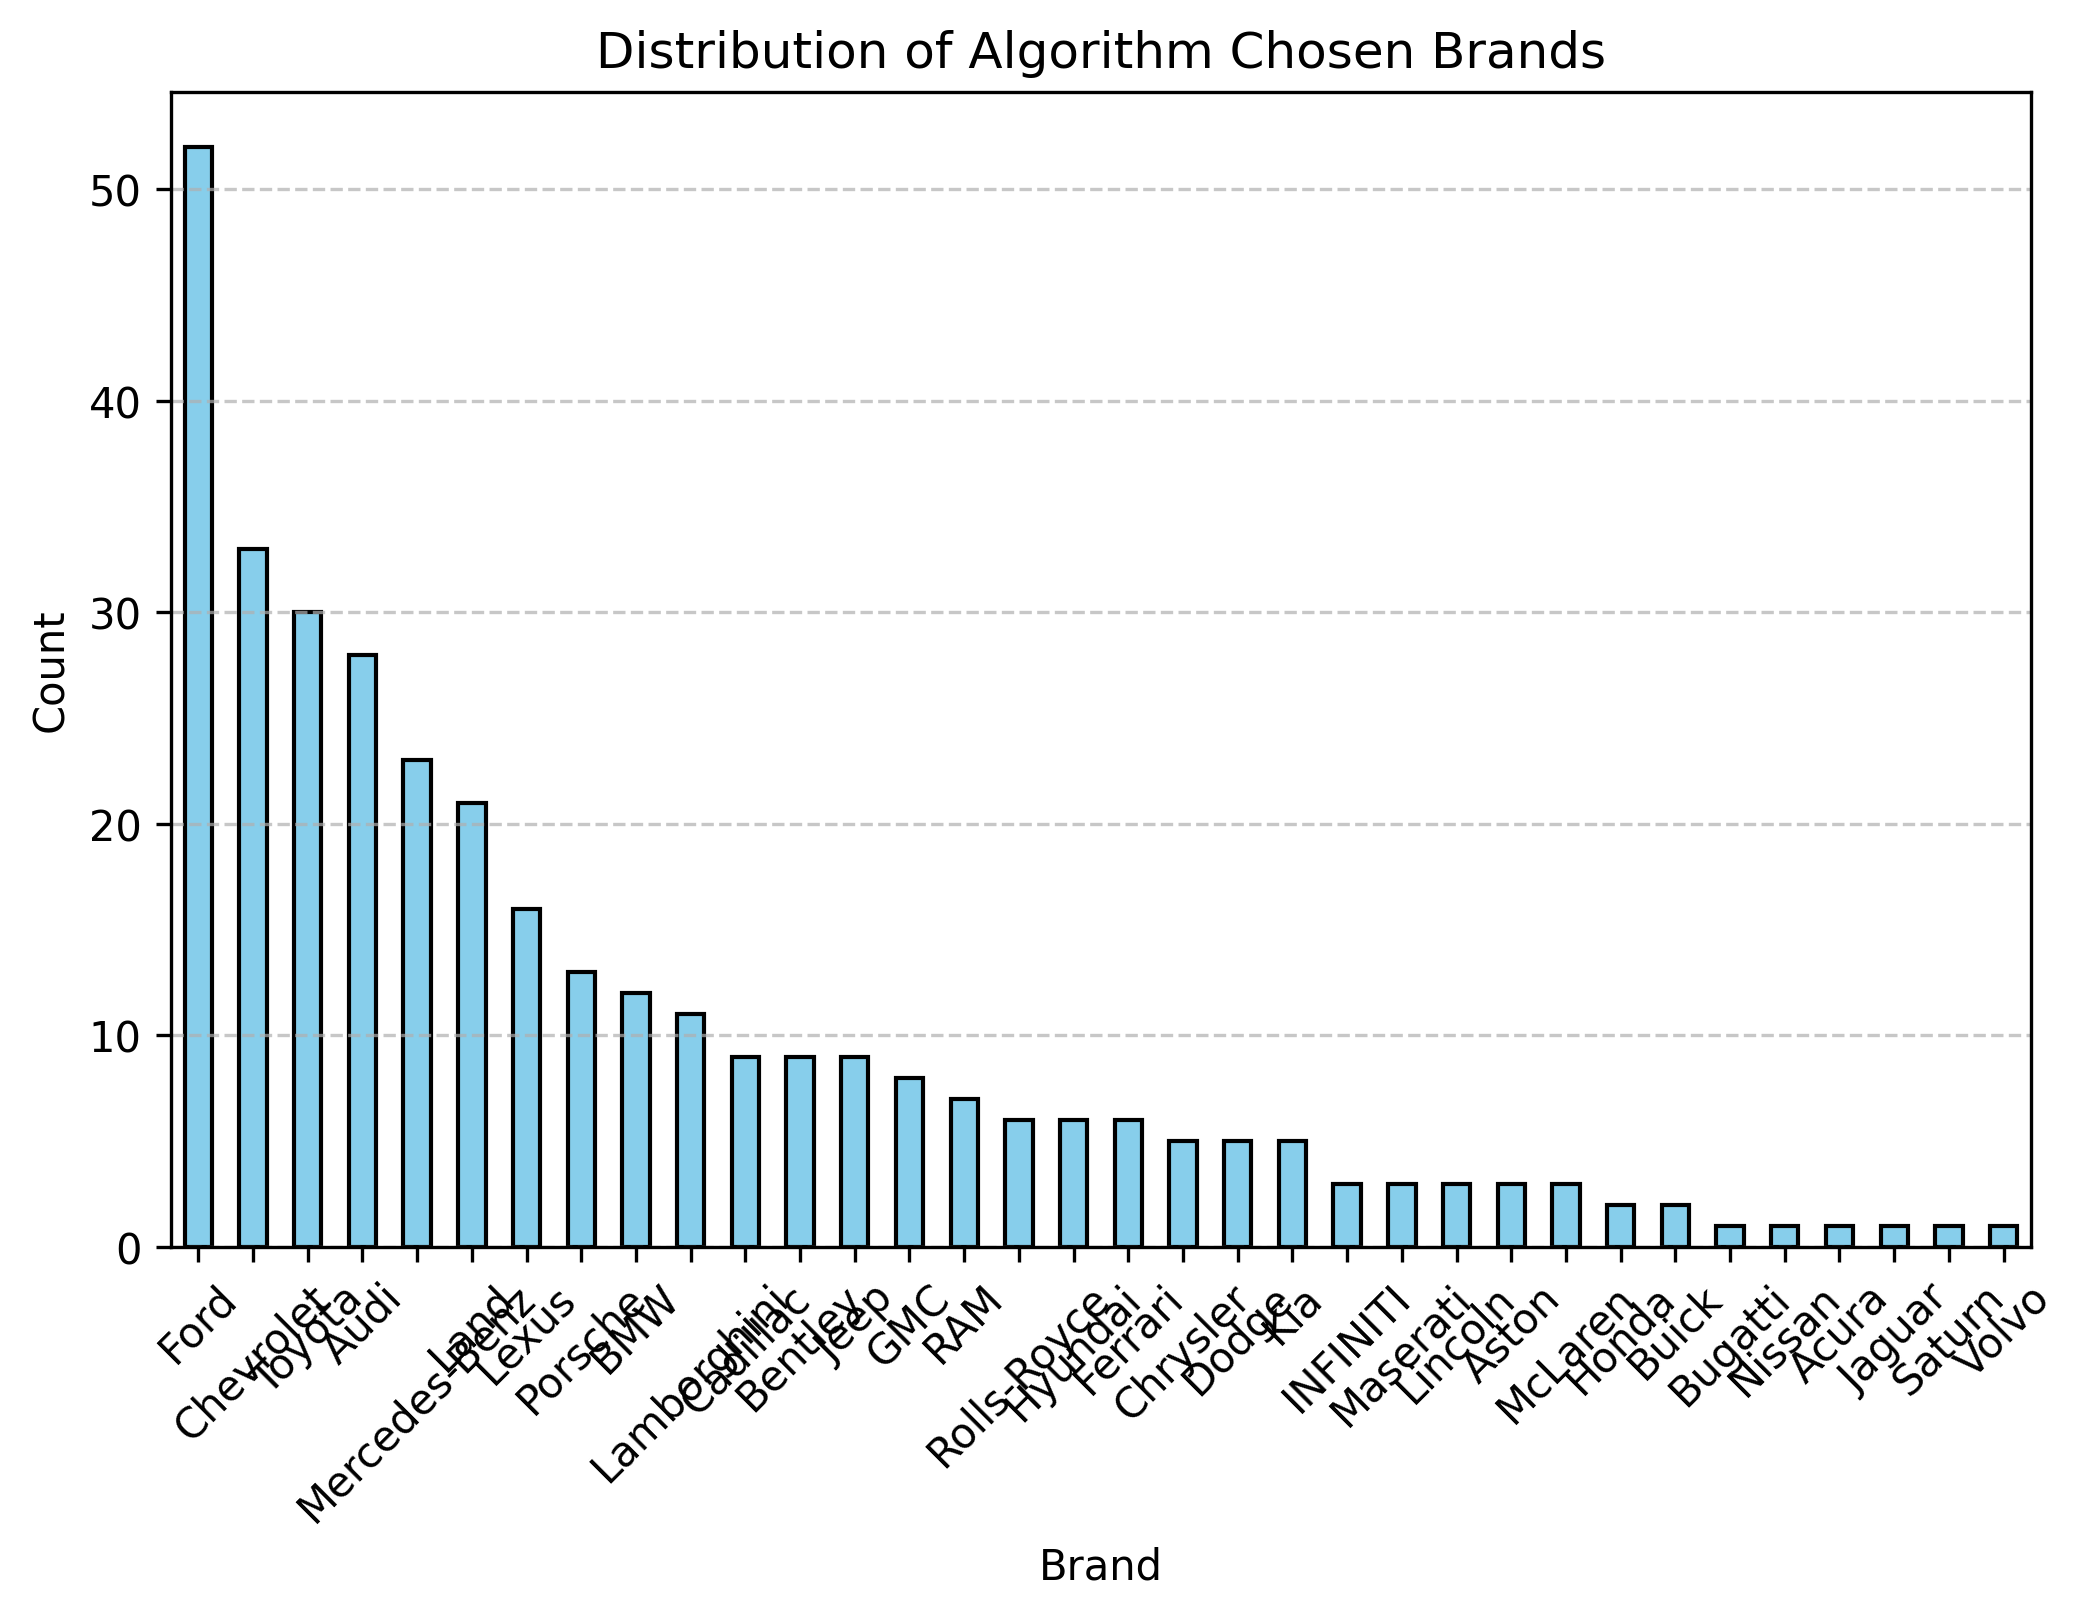
\includegraphics[width=\textwidth]{algo_brand.png}
        \caption{Distribution of car brand from CVXPY}
        \label{fig:algo_brand}
    \end{minipage}\hfill
    \begin{minipage}{0.45\textwidth}
        \centering
        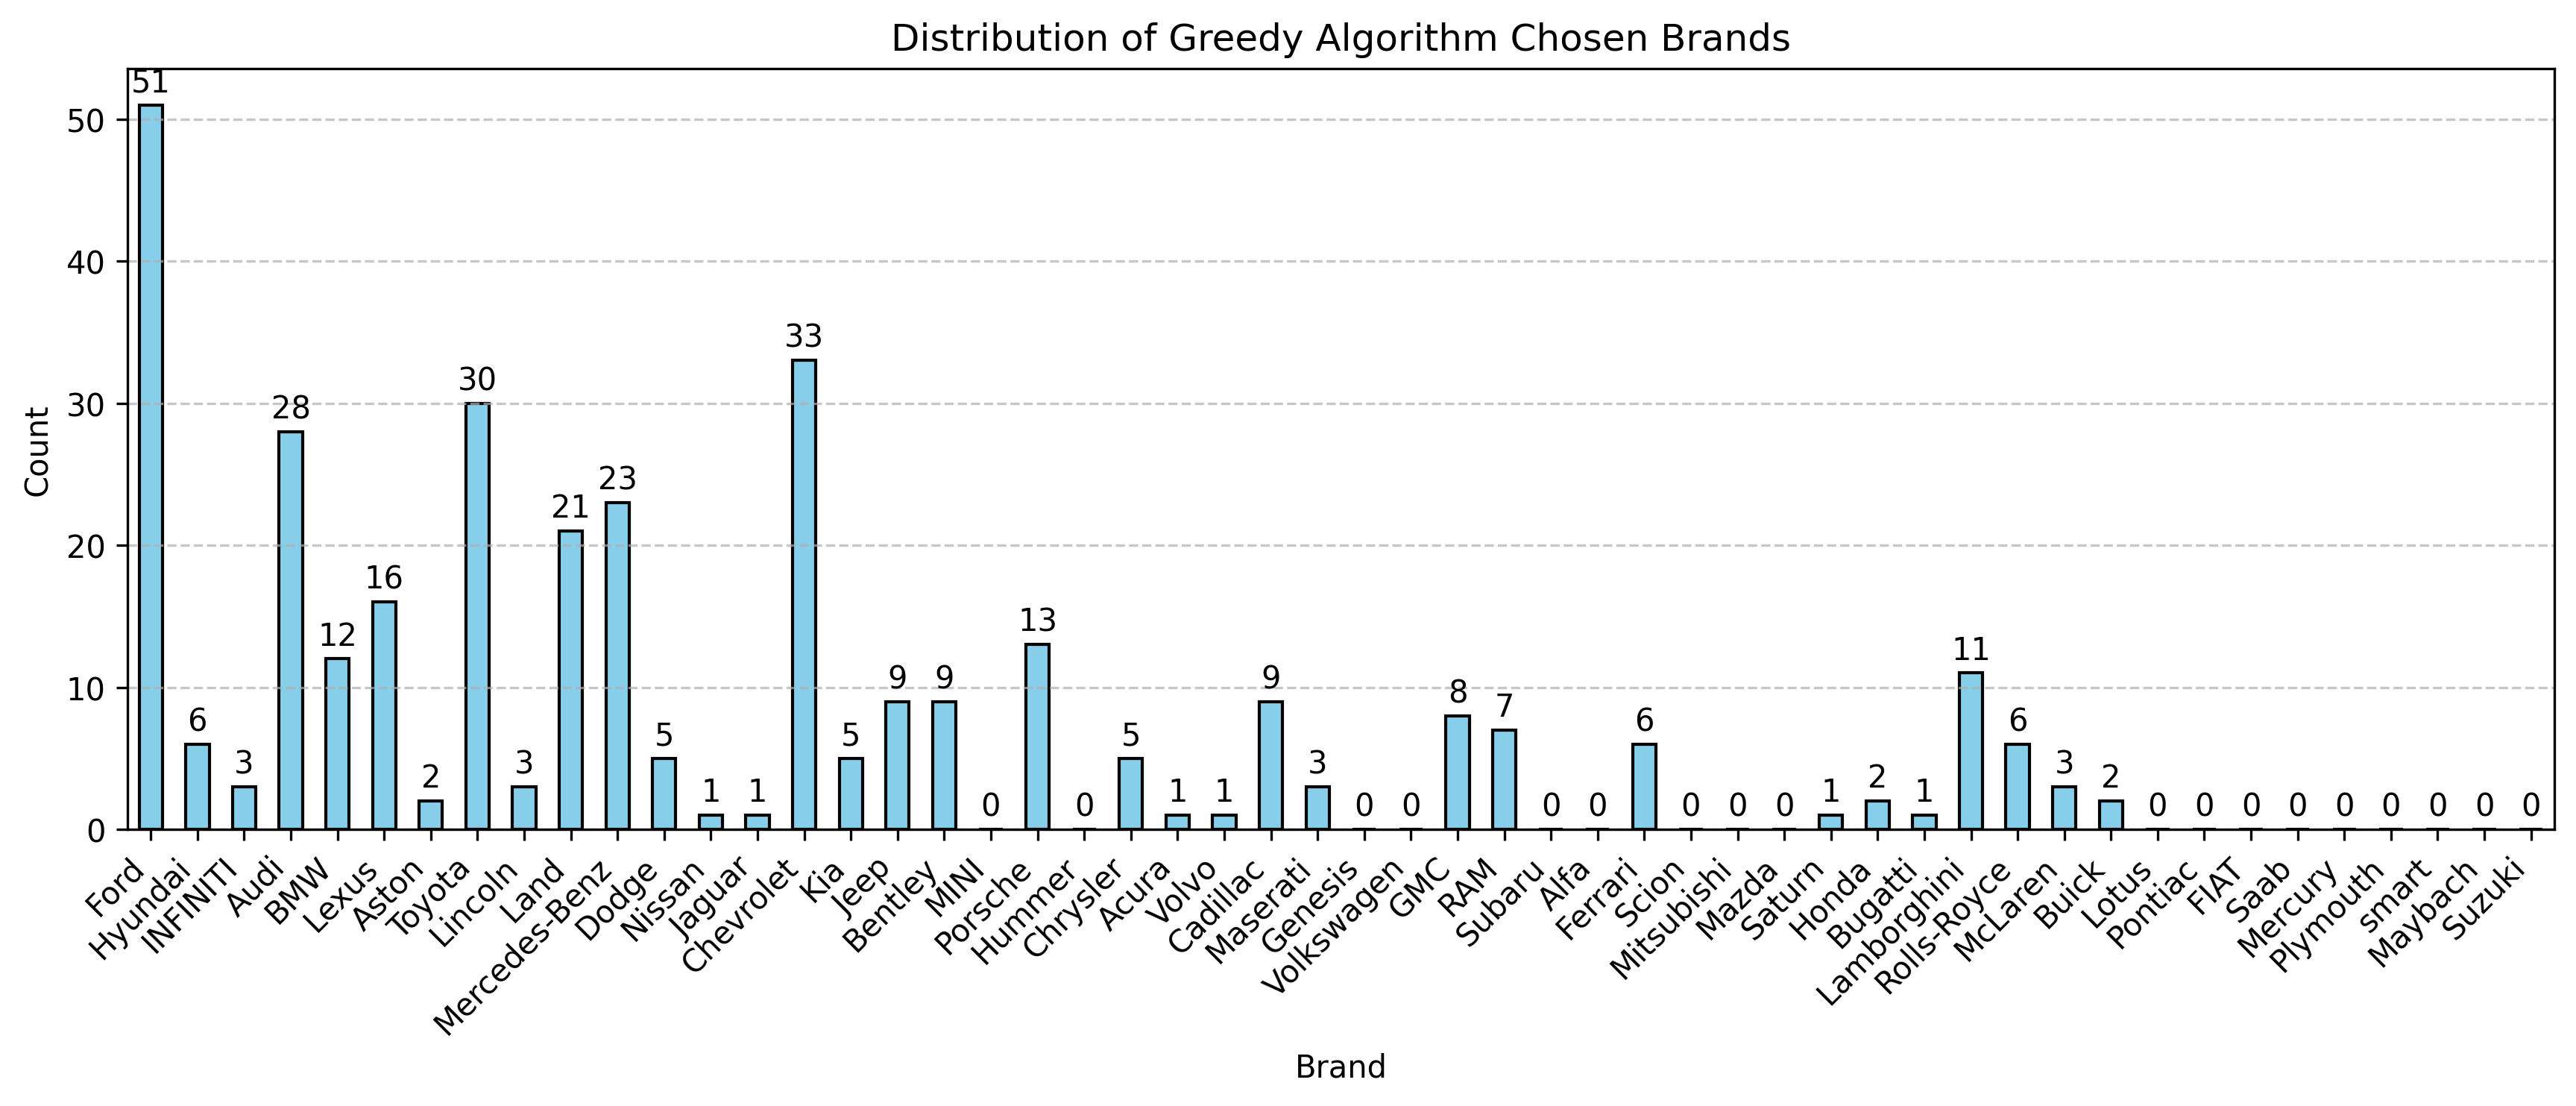
\includegraphics[width=\textwidth]{greedy_budget_brand.png}
        \caption{Distribution of car brand from Budget Algorithm}
        \label{fig:algo_import}
    \end{minipage}\hfill
    \begin{minipage}{0.45\textwidth}
        \centering
        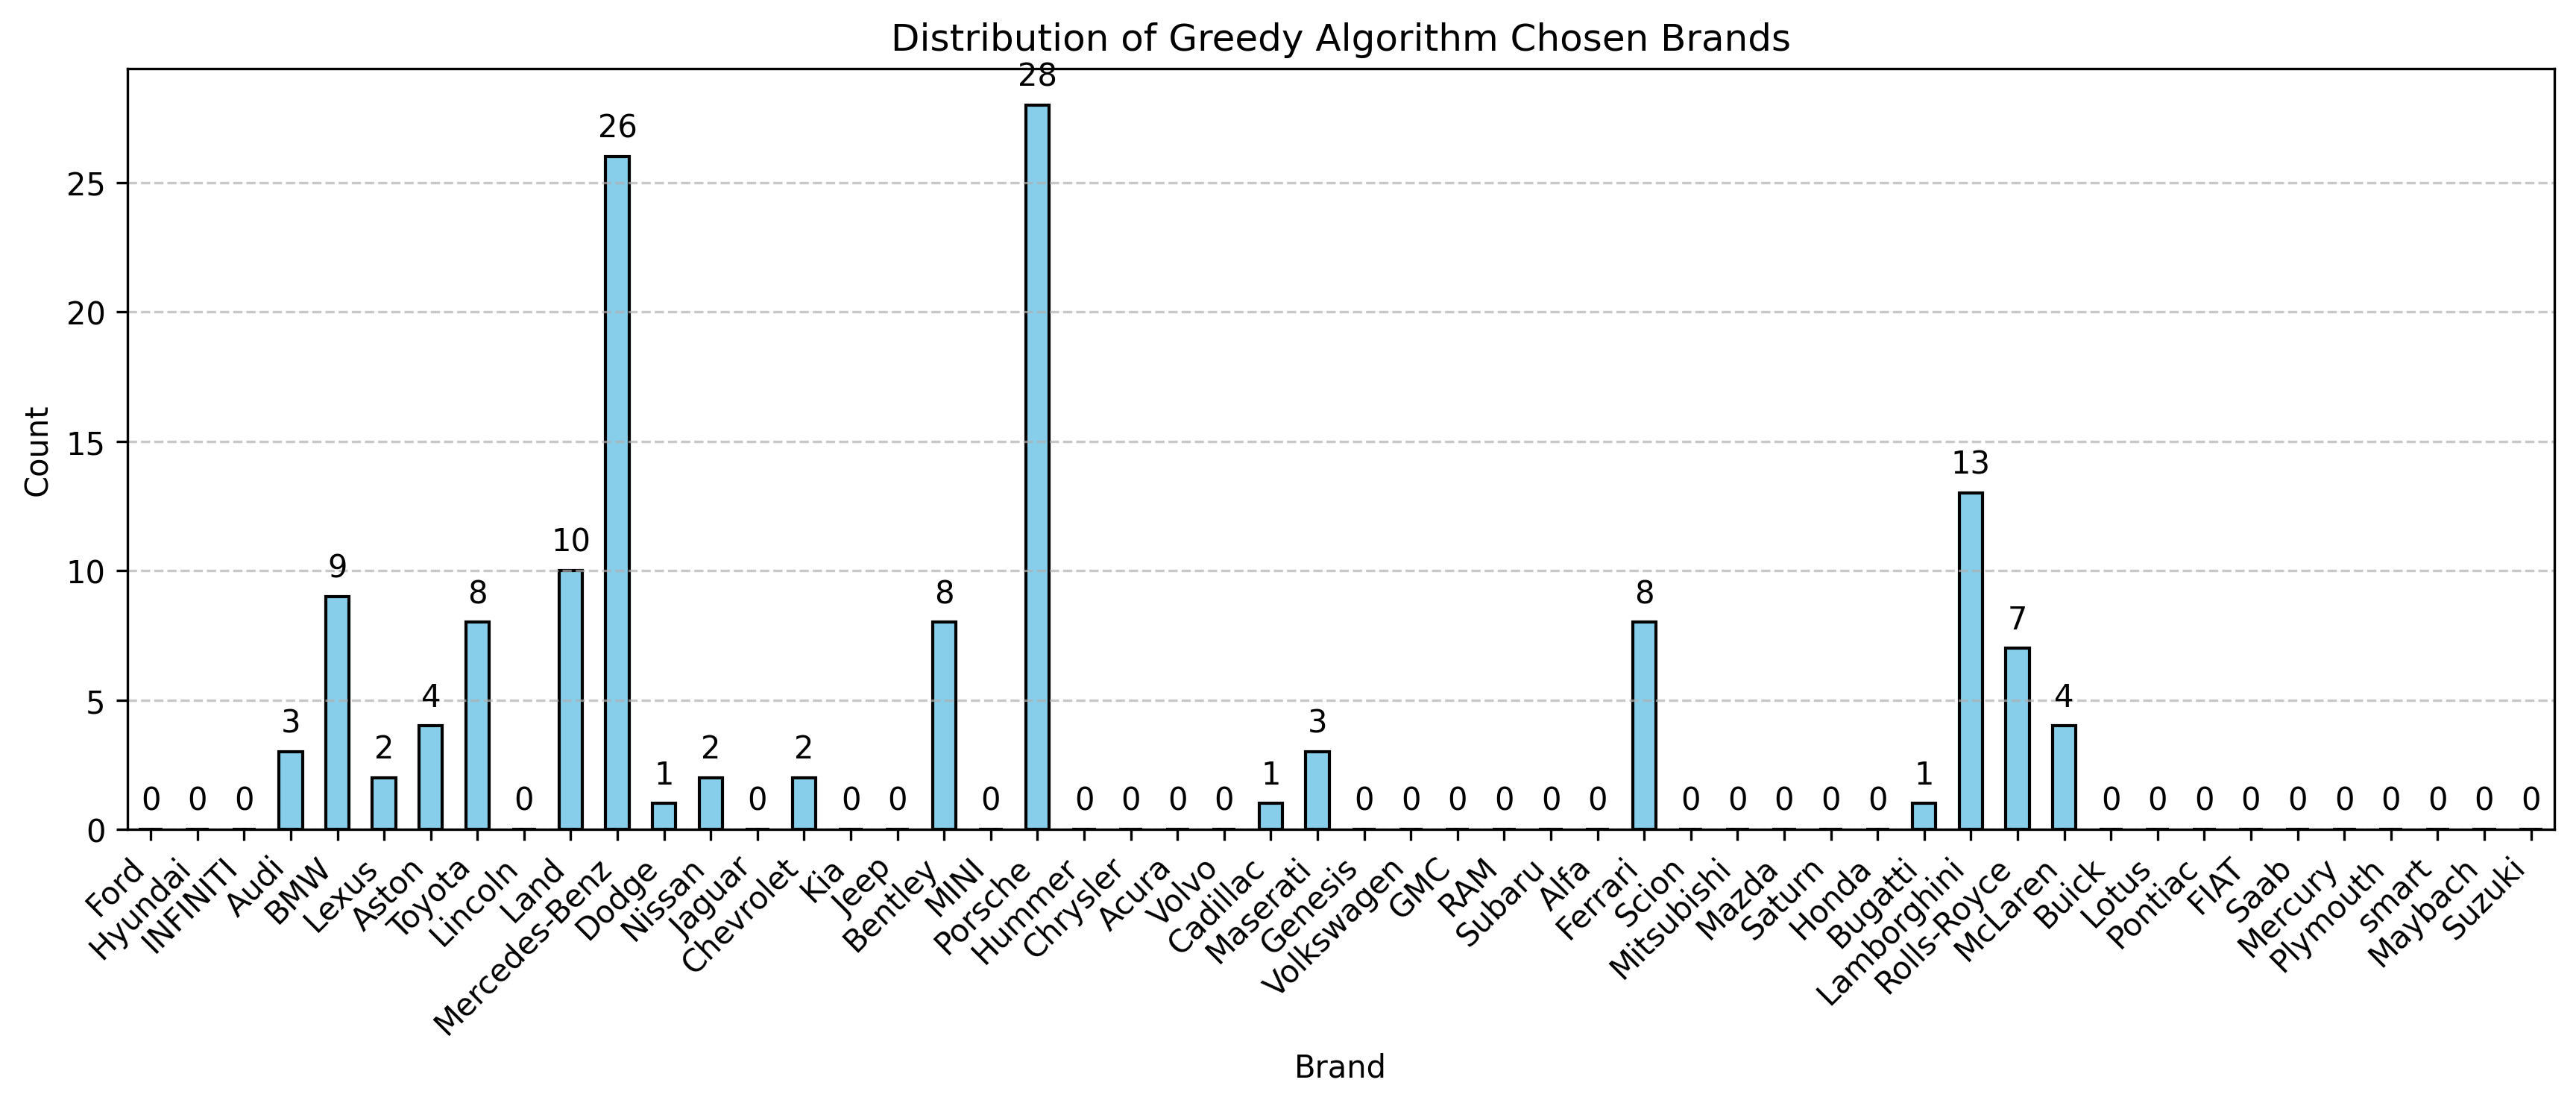
\includegraphics[width=\textwidth]{greedy_size_brand.png}
        \caption{Distribution of car brand from Size Algorithm}
        \label{fig:greedy_budget_import}
    \end{minipage}
\end{figure}

\subsubsection{Compare Performance Between Two Greedy Algorithms}
Based on the analysis above, we conclude that the Budget Algorithm outperforms the Size Algorithm in approximating CVXPY results. This section further explores the performance of the two greedy algorithms by varying the budget constraint and parking lot size constraint. \par
We first analyzed the sensitivity of both algorithms to changes in the budget constraint. As shown in Figure 12, the performance gap between the Budget Algorithm and the Size Algorithm diminishes as the available budget increases, and their output eventually converge at around when the budget is at $\$$96 million.  \par
Interestingly, when testing the sensitivity by varying the size constraint, we observed that the outputs of both algorithms remained constant as the available parking lot size increased from the initial condition stated in the problem to the total size of all possible cars (shown in Fig. 13).  \par
This unexpected result prompted further investigation. By examining the algorithm outputs across a range of available sizes from 0 to the total size of all cars, we found that the output remained stable starting at an available size of 5000 \(m^2\), where the Budget Algorithm performs better than Size Algorithm does (shown in Fig. 14).  \par
This indicates that when the total size constraint exceeds a certain threshold, it can be safely omitted from the optimization process.\par
\begin{figure}[h]
    \centering
    \begin{minipage}{0.45\textwidth}
        \centering
        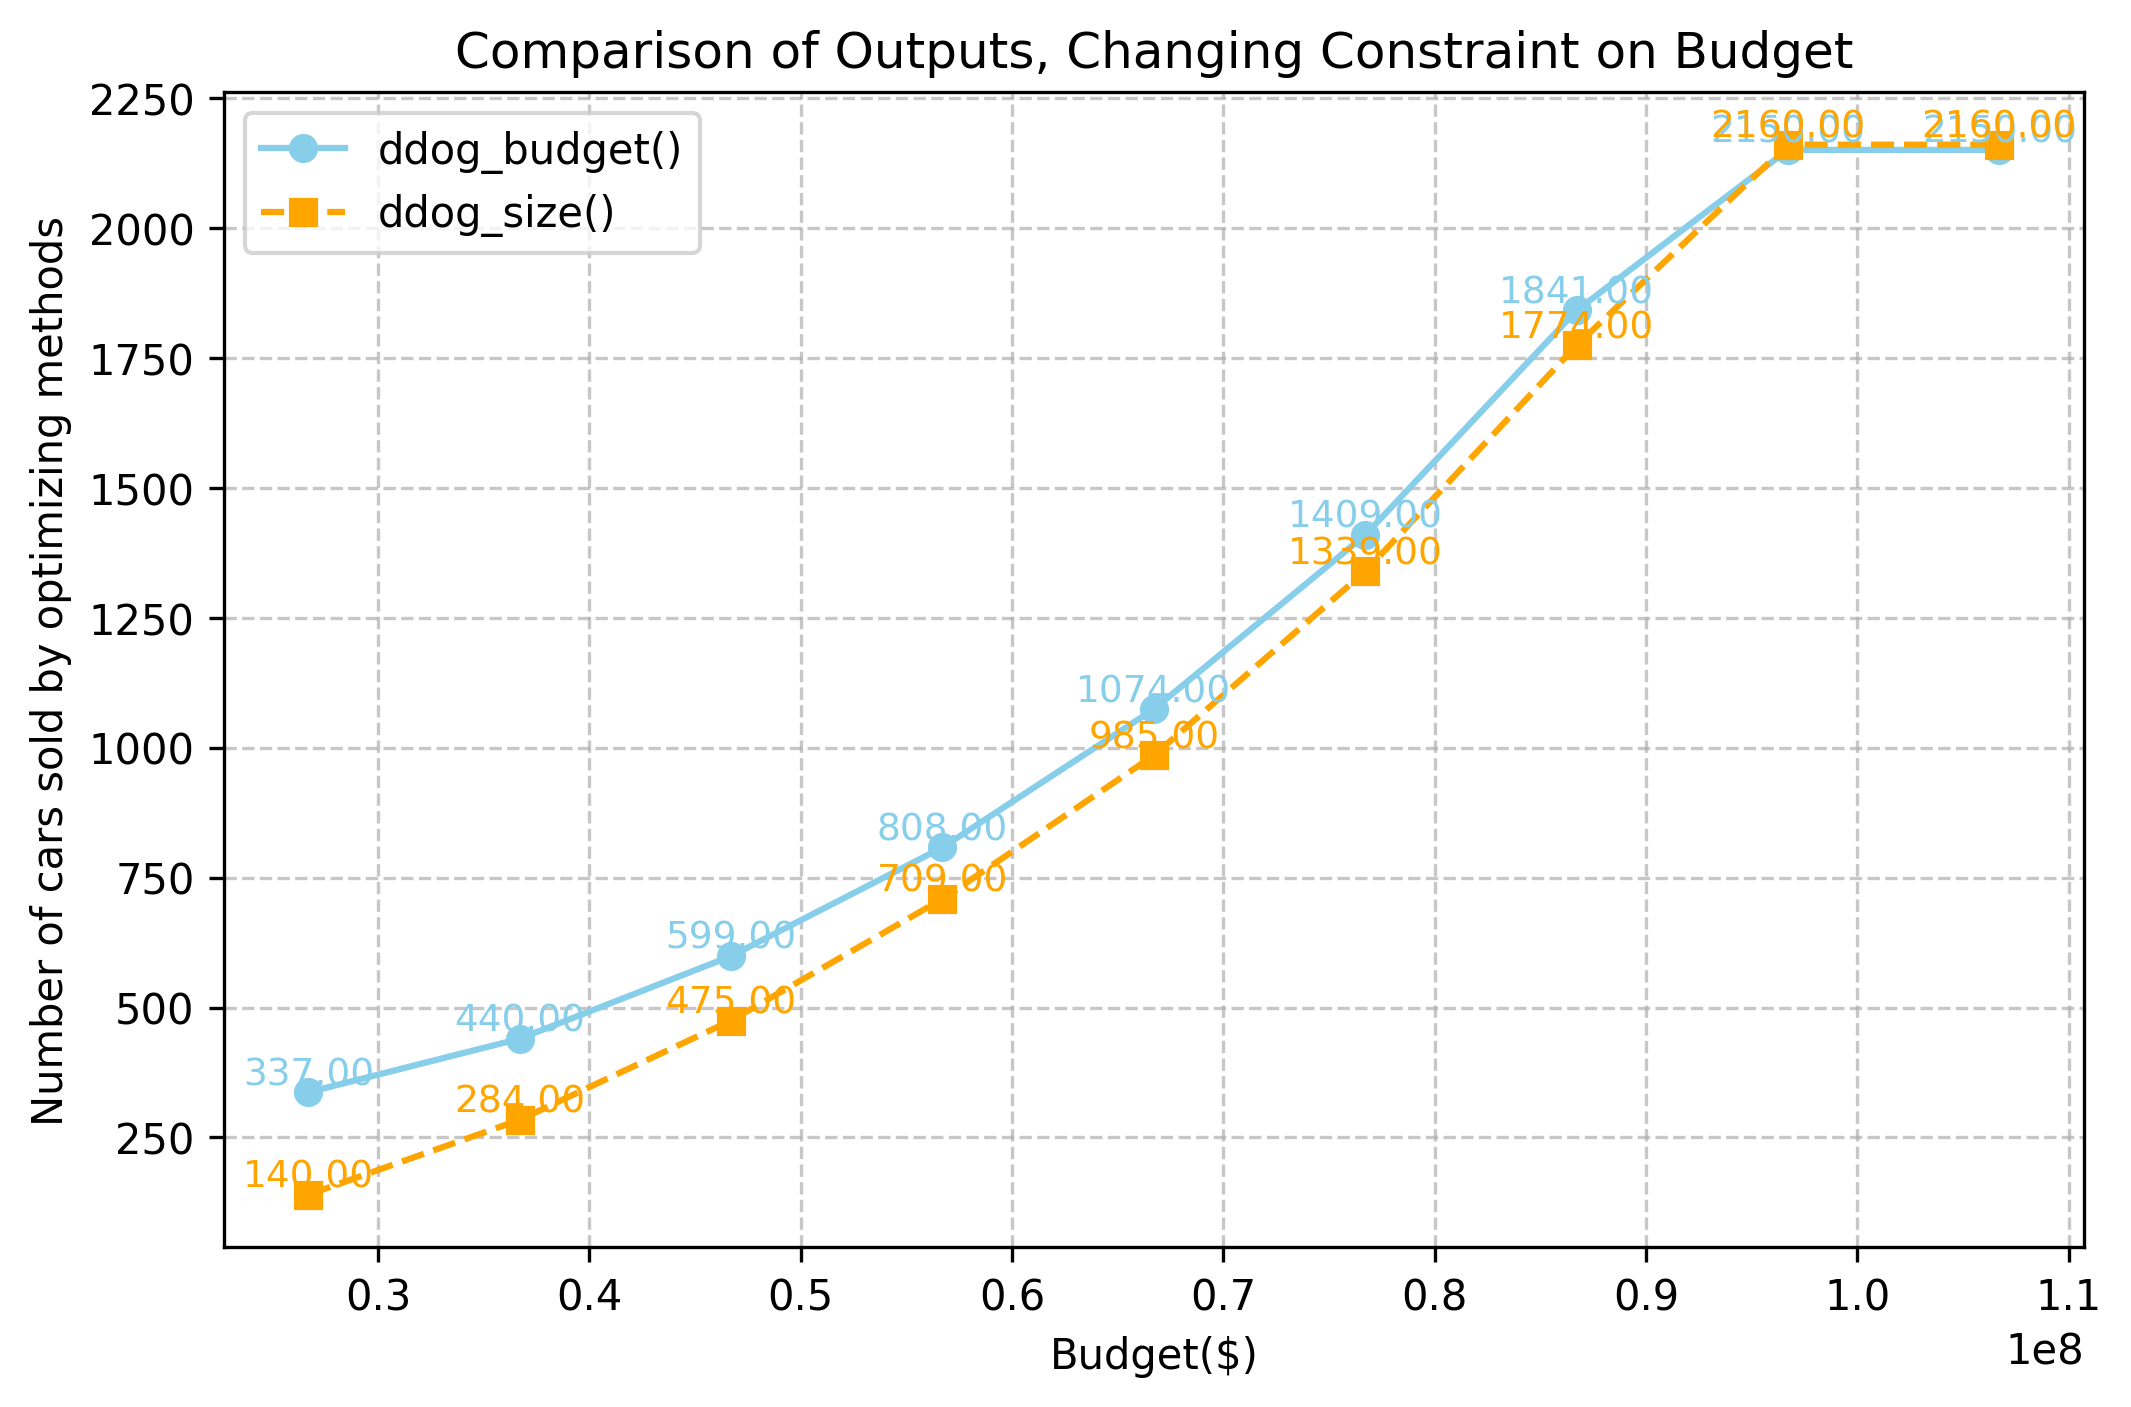
\includegraphics[width=\textwidth]{compare_budget.png}
        \caption{Distribution of car brand from CVXPY}
        \label{fig:compare_budget}
    \end{minipage}\hfill
    \begin{minipage}{0.45\textwidth}
        \centering
        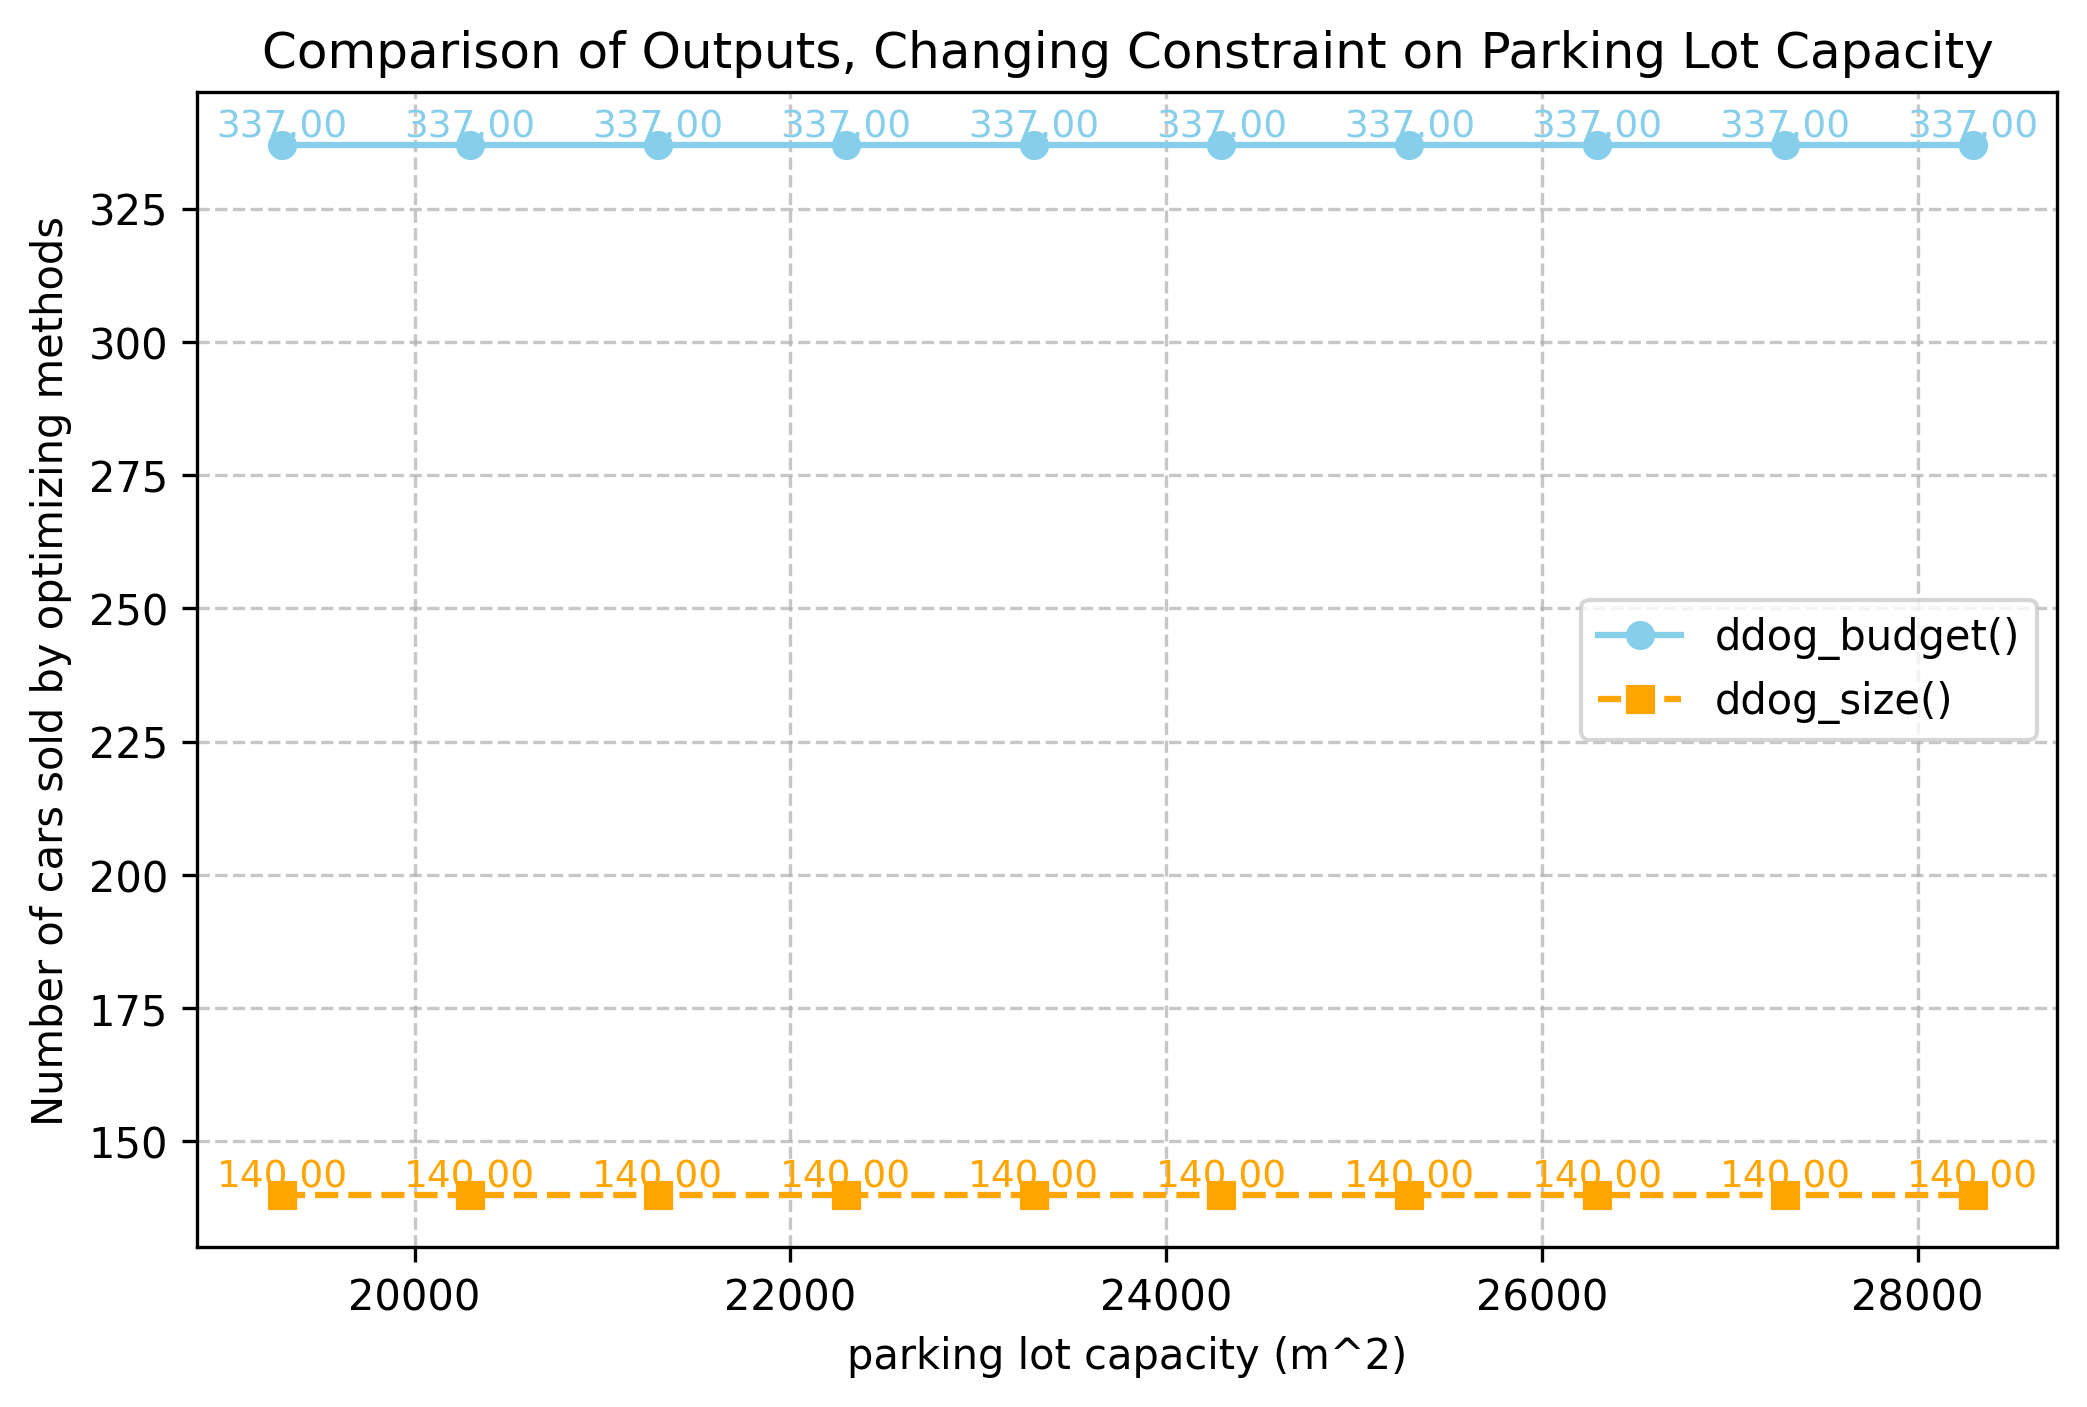
\includegraphics[width=\textwidth]{compare_capacity.png}
        \caption{Distribution of car brand from Budget Algorithm}
        \label{fig:compare_capacity}
    \end{minipage}\hfill
    \begin{minipage}{0.45\textwidth}
        \centering
        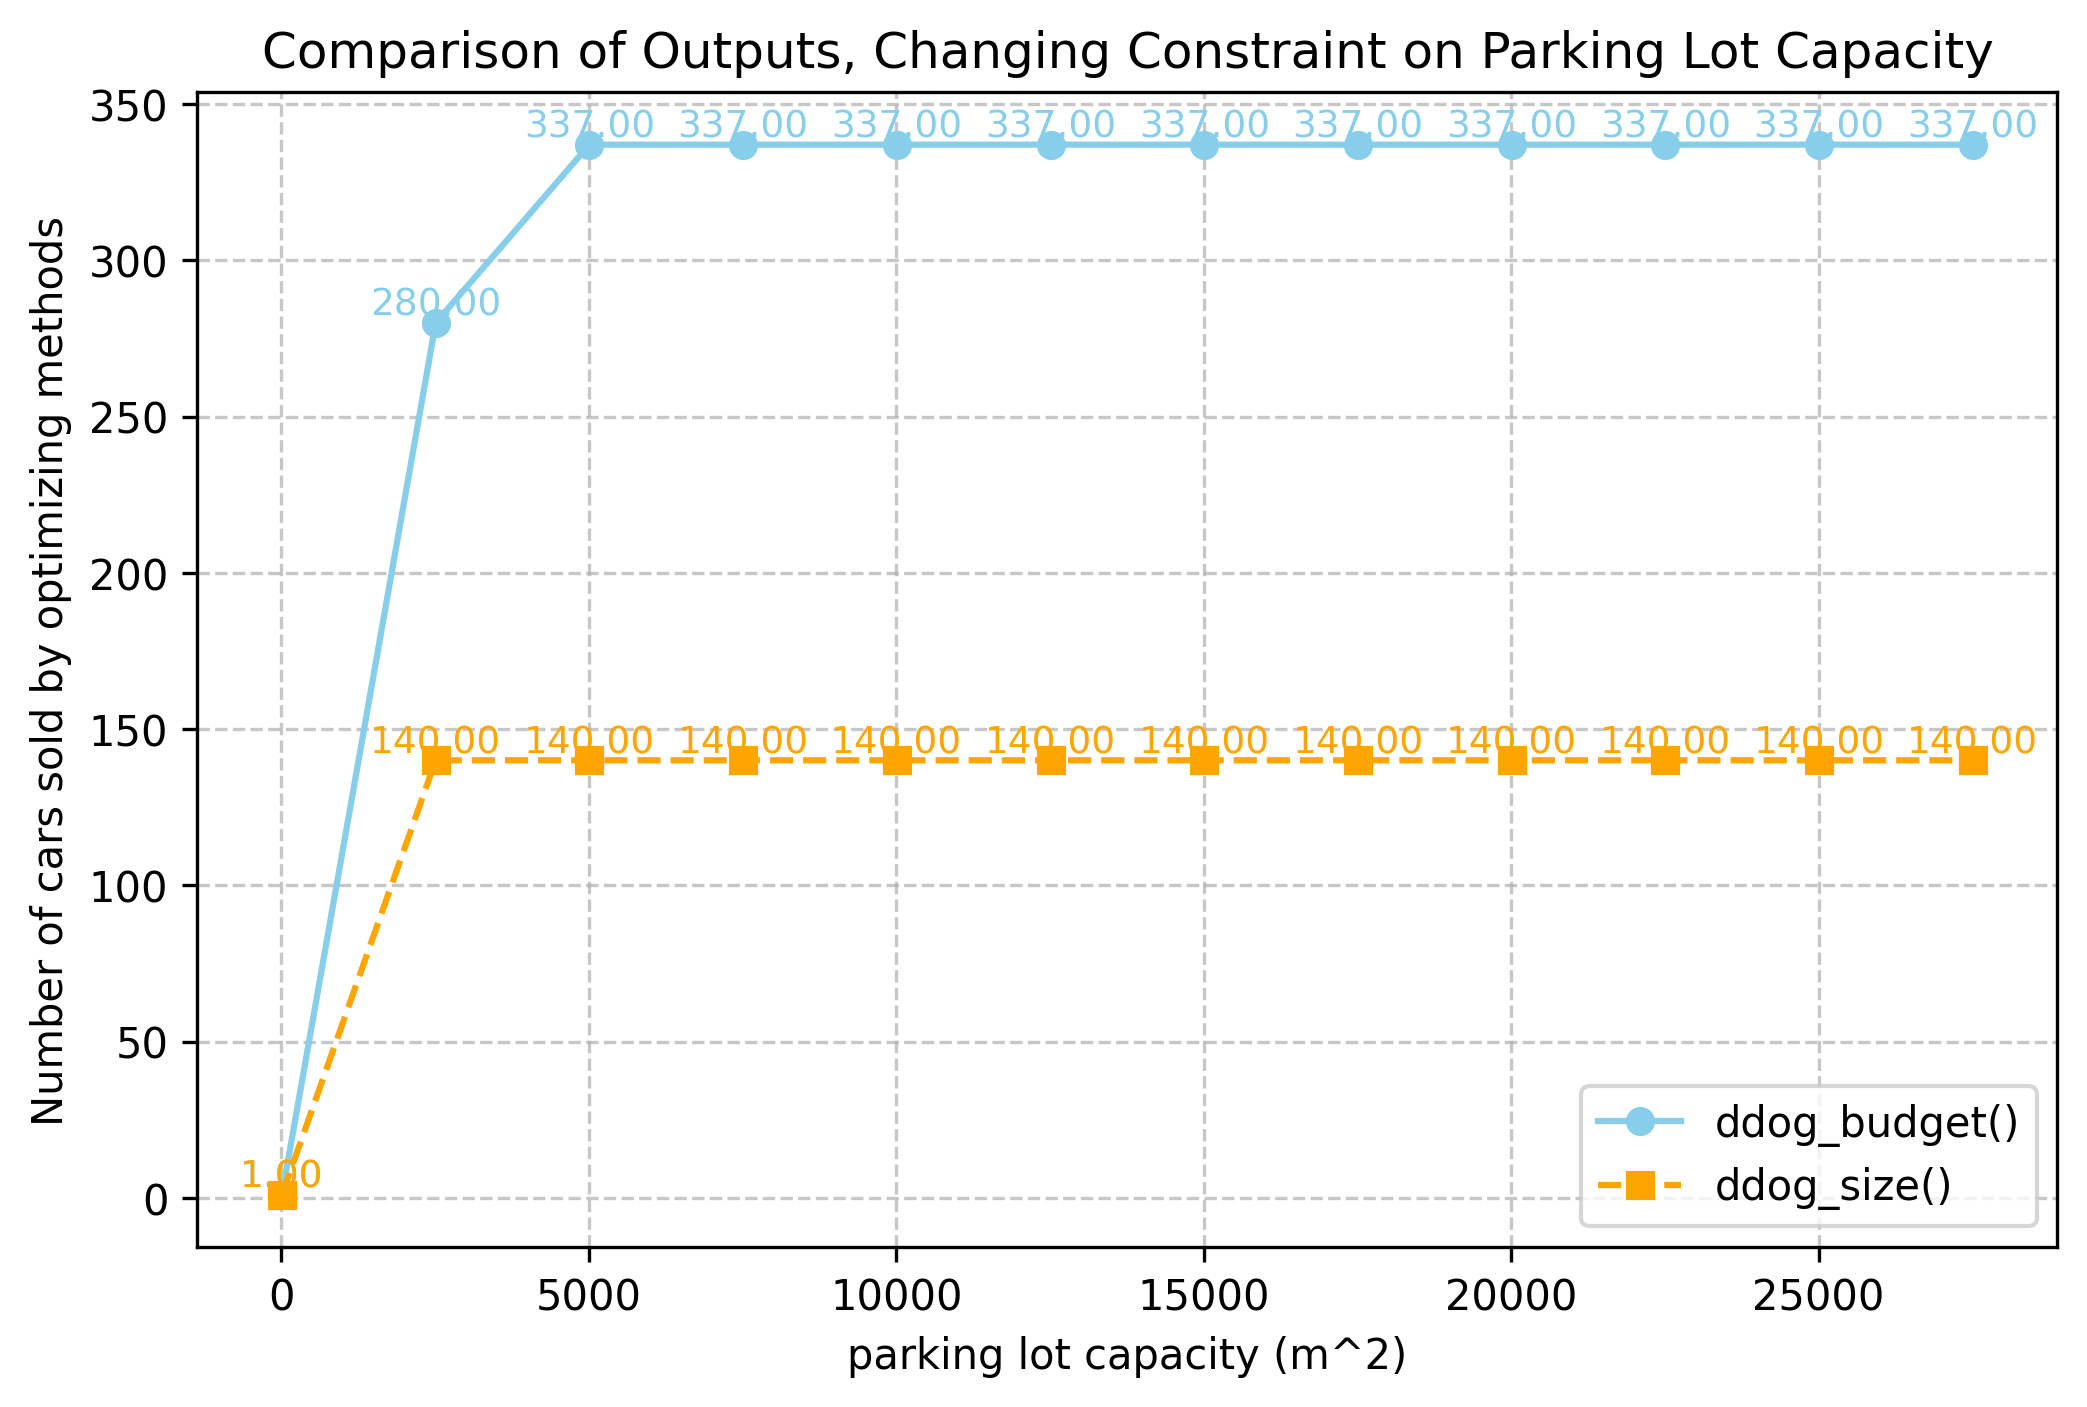
\includegraphics[width=\textwidth]{compare_capacity_2.png}
        \caption{Number of Cars sold by two greedy algorithms, varying parking lot size constraint from zero to total size of all available cars}
        \label{fig:compare_capacity_2}
    \end{minipage}
\end{figure}

\subsection{Discussion and Future Improvements}

While the project’s optimization framework provides a solution for dealership inventory selection, there are several areas can be further improved to enhance its applicability and reliability in real-world decision-making. This section will discusses about potential improvements based on data accuracy, alternative modeling methods, and some extra constraints that could be incorporated into future operations of the model.

\begin{enumerate}
    \item \textbf{Refining Vehicle Size and Parking Constraints:} 
One of the key limitations of the current optimization model is the approximation of vehicle sizes. Due to the lack of precise parking space requirements in the dataset, the top-down area of vehicles was estimated based on rough car dimensions. Future refinements could apply actual vehicle dimensions sourced from different manufacturer specifications or dealership historical data records to provide a more trustworthy and precise spatial constraint formulation. Moreover, this optimization model possesses an assumption of a uniform layout of the parking lot, whereas the real-world dealership has irregular parking lot shapes and sizes, and other limitations such as reserved lot, and structural obstructions. Enhancing the parking constraints to reflect these real-world conditions may help to improve the optimization model's practical applicability.

    \item \textbf{Enhancing Cost Modeling:}
The current optimization assumes that the vehicles’ price is determined by a depreciation factor applied to the market price. While this formula does provide a reasonable estimate price, the actual auction prices can be highly varied and dependent on external market conditions. The future operations of the optimization model could utilize real auction price distributions, allowing for a more accurate representation of dealership sourcing costs. Additionally, any cost related to vehicle refurbishment, transportation, and dealership-specific fees could be account to better approximate net profit margins.

    \item \textbf{Multi-Objective Optimization for Strategic Decision-Making
    :} 
The current optimization model is solely solved to maximize profits while considering spatial and financial constraints. However, real-world dealerships may have additional strategic goals related to their business development, such as maintaining a diverse inventory to attract a broad customer group or prioritizing eco-friendly vehicles to comply with sustainability promotion. Future improvements could explore multi-objective optimization, where trade-offs between profitability, environmental impact (e.g. carbon tax), and inventory diversity are explicitly considered.

    \item \textbf{Algorithmic Efficiency and Scalability:}
The current optimization model leverages integer linear programming (ILP) using CVXPY as well as a greedy heuristic to approximate solutions. Althoughugh the ILP approach guarantees an optimal solution, it may become computationally expensive as tdata set set grows. Future work could explore metaheuristic approaches, such as genetic algorithms, simulated annealing, or particle swarm optimization, which can provide near-optimal solutions with lower computational costs. 


    \item \textbf{Expanding More Possible Constraints for Real-world Dealership Business Operations:}
    Beyond spatial and financial constraints, dealerships often face regulatory and operational limitations. In order to get a more realistic revenue, future optimization models could include:
\begin{itemize}
    \item Vehicle age restrictions, where certain dealerships may only accept vehicles under a specific year.
    \item Brand distribution strategies, ensuring that a dealership maintains a balanced mix of high-end and budget-friendly cars.
    \item Introducing financing and loan structures, where capital allocation for vehicle purchases is constrained by financing agreements.
    \item Customer preference modeling, investigate sales history data to predict the likelihood of selling specific vehicle types within a given timeframe.
\end{itemize}
\end{enumerate}

\section{Conclusion}
The optimal maximum total profit is \$8,301,576.50. Our combinatorial programming model effectively identifies the optimal strategy for solving the knapsack problem. The results highlight how mathematical optimization can guide decision-making in inventory management for a car dealership scenario.  \par
The comparison between the CVXPY algorithm and the greedy algorithms, particularly the Size Algorithm, illustrates the advantages of a comprehensive optimization approach over a locally focused decision-making strategy. While the Budget Algorithm approximates the CVXPY result with good accuracy, it still deviates from the actual CVXPY outcome.\par
CVXPY prioritizes hybrid and flex-fuel vehicles, integrating economic and environmental factors more effectively. Although all algorithms recognize profitability trends between imported and domestic cars, CVXPY optimizes inventory with a more comprehensive strategy.


\newpage
\begin{thebibliography}{9}
\bibitem{KaggleDataset} 
Taeef Najib. (2023). Used Car Price Prediction Dataset. Retrieved from \url{https://www.kaggle.com/datasets/taeefnajib/used-car-price-prediction-dataset/data}.
\end{thebibliography}


\end{document}
